\documentclass[
  %paper=23.9cm:16.9cm, %Actual book size
  paper=a4paper,
  pagesize,
  twoside,
  10pt,
  chapterprefix,
  headsepline=on,
  footinclude=off,
  DIV=18,
  BCOR=7mm,
  bibliography=totoc,
  numbers=noenddot,
  open=right,
]{book}
\usepackage[%
  %papersize={23.9cm,16.9cm},
  paperwidth=16.9cm, 
  paperheight=23.9cm,
  left=20mm,
  right=20mm,
  top=25mm,
  bottom=25mm,
]{geometry}

\synctex=1                    % instead of "pdflatex -synctex=1 main"
\usepackage[,numfigreset=1,mathnumfig]{sphinx}
%\makenomenclature

\usepackage{lipsum}           % generating fill-in text for this thesis template

\usepackage{ifthen}           % if-then-else (to choose PhD/Lic titles)

\usepackage[utf8]{inputenc}   % unicode letters in the input tex document

\usepackage[T1]{fontenc}      % unicode letters in the output pdf

\usepackage{amssymb, amsmath} % math symbols
\usepackage{microtype}        % micro typesetting (on errors use draft to disable)

\usepackage{booktabs}         % better table formatting

\usepackage[pdftex]{graphicx} % images

\usepackage{tikz}             % simply amazing graphics library for LaTeX
\usetikzlibrary{calc}
\usetikzlibrary{matrix}

%%% Flow chart stuff:
\usepackage{tikz}
\usetikzlibrary{shapes.geometric, arrows}
\tikzstyle{startstop} = [rectangle, rounded corners, minimum width=2cm, minimum height=1cm,text centered, draw=black, fill=red!30]
\tikzstyle{io} = [rectangle, rectangle, minimum width=0.0cm, minimum height=0.7cm, draw=none, fill=white]
\tikzstyle{process} = [rectangle, minimum width=1cm, minimum height=1cm, text centered, draw=black, fill=orange!30]
\tikzstyle{decision} = [diamond, minimum width=3cm, minimum height=0.7cm, text centered, draw=black, fill=green!30]
\tikzstyle{arrow} = [thick,->,>=stealth]
\tikzstyle{white-box} = [rectangle, minimum width=2cm, minimum height=0.7cm, text centered, draw=black, fill=white]
\tikzstyle{black-box} = [rectangle, minimum width=2cm, minimum height=0.7cm, text centered, draw=black, fill=black, text=white]
\tikzstyle{grey-box} = [rectangle, minimum width=2cm, minimum height=0.7cm, text centered, draw=black, fill=gray, text=black]

\makeatletter
\tikzset{
    database top segment style/.style={draw},
    database middle segment style/.style={draw},
    database bottom segment style/.style={draw},
    database/.style={
        path picture={
            \path [database bottom segment style]
                (-\db@r,-0.5*\db@sh) 
                -- ++(0,-1*\db@sh) 
                arc [start angle=180, end angle=360,
                    x radius=\db@r, y radius=\db@ar*\db@r]
                -- ++(0,1*\db@sh)
                arc [start angle=360, end angle=180,
                    x radius=\db@r, y radius=\db@ar*\db@r];
            \path [database middle segment style]
                (-\db@r,0.5*\db@sh) 
                -- ++(0,-1*\db@sh) 
                arc [start angle=180, end angle=360,
                    x radius=\db@r, y radius=\db@ar*\db@r]
                -- ++(0,1*\db@sh)
                arc [start angle=360, end angle=180,
                    x radius=\db@r, y radius=\db@ar*\db@r];
            \path [database top segment style]
                (-\db@r,1.5*\db@sh) 
                -- ++(0,-1*\db@sh) 
                arc [start angle=180, end angle=360,
                    x radius=\db@r, y radius=\db@ar*\db@r]
                -- ++(0,1*\db@sh)
                arc [start angle=360, end angle=180,
                    x radius=\db@r, y radius=\db@ar*\db@r];
            \path [database top segment style]
                (0, 1.5*\db@sh) circle [x radius=\db@r, y radius=\db@ar*\db@r];
        },
        minimum width=2*\db@r + \pgflinewidth,
        minimum height=3*\db@sh + 2*\db@ar*\db@r + \pgflinewidth,
    },
    database segment height/.store in=\db@sh,
    database radius/.store in=\db@r,
    database aspect ratio/.store in=\db@ar,
    database segment height=0.1cm,
    database radius=0.25cm,
    database aspect ratio=0.35,
    database top segment/.style={
        database top segment style/.append style={#1}},
    database middle segment/.style={
        database middle segment style/.append style={#1}},
    database bottom segment/.style={
        database bottom segment style/.append style={#1}}
}
\makeatother
%\usepackage[%                 %
%  a4paper%
%  ,twoside                    %
%  ,inner=2.5cm                % inner margin
%  ,outer=2.5cm                % outer margin
%  ,bindingoffset=1cm       % additional binding offset on the inner side
%  ,bottom=3cm
%]{geometry}                   % Adjust the margins

\usepackage{fancyhdr}         % fine-tuning of headers
\pagestyle{fancy}

\usepackage{emptypage}        % no page numbers in headers/footers of blank pages between chapters

%\usepackage{setspace}         % for \setstretch in captions

\usepackage[%
    margin=0.75cm,            % make captions narrower than the main text
    font={small,stretch=0.80}%%
  ]{caption}                  % captions

\usepackage{subcaption}       % subcaption -- subfigures (replaces subfig)

\usepackage{url}              % handles URLs correctly (e.g. DOI, software links)
% % % Biblatex
\usepackage[%
  url=true,%                  % print URLs in references, except for the ones removed below
  backend=biber,%             % use biber instead of bibtex
  style=apa,%          % cite as: (Author 2008)
%  maxbibnames=10,%            % max names in bibliography
   maxcitenames=2,%            % max names in citation
   maxbibnames=99,
   giveninits=true,
   date=year,
%  mincitenames=1,%            % if there are more than maxcitenames, shrink to this
%  backref=true,%              % prints page numbers (wrong with \frontmatter and hypertexnames=false)
  dashed=false,                % do not replace repeated author with a dash in bibliography
  uniquename=false,           % So not distinguish people with same family name by adding initial
  isbn=true,
]{biblatex}                   % Modern bibtex replacement (bibliography mgmt)
\addbibresource{library.bib}  % Bibliography file

% Macro to add URL:\entryneedsurl{citename}
\DeclareBibliographyCategory{needsurl}
\newcommand{\entryneedsurl}[1]{\addtocategory{needsurl}{#1}}
\renewbibmacro*{url+urldate}{%
  \ifcategory{needsurl}
    {\printfield{url}%
     \iffieldundef{urlyear}
       {}
       {\setunit*{\addspace}%
        \printurldate}}
    {}}
\entryneedsurl{imo_standards_2002}
\entryneedsurl{ittc_maneuvering_2008}
\entryneedsurl{matusiak_dynamics_2021}
\entryneedsurl{piehl_ship_2016}
\entryneedsurl{himeno_prediction_1981}
\entryneedsurl{ikeda_velocity_1979}


%\DeclareNameAlias{author}{last-first}
%\DeclareCiteCommand{\fullcite}
%  {\usebibmacro{prenote}}
%  {\usedriver
%     {\defcounter{minnames}{6}%
%      \defcounter{maxnames}{6}}
%     {\thefield{entrytype}}.}
%  {\multicitedelim}
%  {\usebibmacro{postnote}}

% Remove URLs from common (easy-to-find) entries.
%\AtEveryBibitem{%
%  \ifboolexpr%
%    {%
%      test { \ifentrytype{book} }
%      or
%      test { \ifentrytype{inbook} }
%      or
%      test { \ifentrytype{inproceedings} }
%      or
%      test { \ifentrytype{incollection} }
%      or
%      test { \ifentrytype{article} }
%    }
%    {\clearfield{url}}
%    {}%
%}
%\AtEveryBibitem{% Clean up the bibtex rather than editing it
% \clearlist{address}
% \clearfield{isbn}
% \clearfield{issn}
% \clearfield{month}
% \clearfield{note}
% \clearlist{publisher}
%}
% End Biblatex


\usepackage[%
   pdftex%
  ,hidelinks%
  ,linktoc=all%               % part of a ToC entry to be made into a link (section/page/all)
  ,unicode%
  ,bookmarksopen=true%
  ,bookmarksopenlevel=0
  ,bookmarksnumbered=true
  %,hypertexnames=false,%     % Correct ToC hyperlinks even with chapter counter reset, but broken biblatex backref.
                              % Instead of using hypertexnames=false, use \renewcommand on \theHchapter, 
                              % see http://tex.stackexchange.com/a/6099
  %,draft                     % draft can be used to avoid some strange links errors
]{hyperref}                   % links in pdf document

\usepackage{bookmark}         % Create pdf bookmarks in one go
\usepackage{nomencl}
\usepackage{float}
% This will add the units
%----------------------------------------------
\newcommand{\nomunit}[1]{%
\renewcommand{\nomentryend}{\hspace*{\fill}#1}}
%----------------------------------------------



\def\equationautorefname~#1\null{Eq.~(#1)\null}
\def\figureautorefname~#1\null{Figure~#1\null}
\def\tableautorefname~#1\null{Table~#1\null}

\usepackage{tocloft}  % No page number of appended papers
\usepackage{appendix}

\usepackage[section]{placeins}  % This prevents placing floats before a section.

\usepackage[Sonny]{fncychap}  % Fancy chapter headings
\ChTitleVar{\normalfont\rmfamily\bfseries\large} % Chapter title

% Fonts
\usepackage{lmodern}          % better font
\usepackage{titlesec}

\titleformat{\section}
{\normalfont\rmfamily\bfseries\large}
{\thesection}{1em}{}

\titleformat{\subsection}
{\normalfont\rmfamily\bfseries\normalsize}
{\thesubsection}{1em}{}

\titleformat{\subsubsection}
{\normalfont\rmfamily\bfseries\normalsize}
{\thesubsubsection}{1em}{}

% Fixing vspaces for chapter heading
\makeatletter
\patchcmd{\@makechapterhead}{\vspace*{50\p@}}{\vspace*{-40\p@}}{}{}
\patchcmd{\@makeschapterhead}{\vspace*{50\p@}}{\vspace*{-40\p@}}{}{}
\patchcmd{\DOTI}{\vskip 80\p@}{\vskip -30\p@}{}{}
\patchcmd{\DOTIS}{\vskip 40\p@}{\vskip -30\p@}{}{}
\makeatother
  
% Table of content fonts
\renewcommand\cftchappagefont{\normalfont\rmfamily\bfseries\normalsize}
\renewcommand\cftsecpagefont{\normalfont\rmfamily\bfseries\normalsize}

\usepackage{makecell}  % to get line breaks in table cells
\setlength\parindent{12pt}  % Indent after new line...

\renewcommand{\cite}{\parencite}




% % % New environments

% \newenvironment{env-name}[optional-number-of-args]{insert-before}{insert-after}

% \newenvironment{env-name}[optional-number-of-args][default-args]{insert-before}{insert-after}

\newenvironment{abstract}{
  \begin{center}
    {\bfseries Abstract\par}  % \bfseries - some bold font, \par - end of paragraph (as empty line)
  \end{center}
  \quotation                  % extra indent from left and right
  \noindent
}
{\par\endquotation}

\newenvironment{keywords}%
{{\bfseries Keywords:}}%
{\par}%
% % % End new environments


% Begin page content adjustments for putting more text on pages.
\renewcommand{\topfraction}{.85}       % max fraction of floats at top
\renewcommand{\bottomfraction}{.7}     % max fraction of floats at bottom
\renewcommand{\textfraction}{.15}      % minimal text wrt. figs
\renewcommand{\floatpagefraction}{.66} % fraction for page of floats. floatpagefraction MUST be less than topfraction 
\renewcommand{\dbltopfraction}{.66}    % fit big float above 2-col. text
\renewcommand{\dblfloatpagefraction}{.66}
\setcounter{topnumber}{9}
\setcounter{bottomnumber}{9}
\setcounter{totalnumber}{20}
\setcounter{dbltopnumber}{9}
\widowpenalty=300                             % widow (at the beginning of page)
\clubpenalty=300                              % orphans (at the end of page)
\setlength{\parskip}{0ex plus 0.5ex}  % space between paragraphs
% End page content adjustments

% % %
% Begin remove page numbers from the "Part I" pages
\fancypagestyle{veryempty}{% no headers, no page numbers
  \fancyhf{} % remove everything
  \fancyfoot{}
  \renewcommand{\headrulewidth}{0pt} % remove lines as well
  \renewcommand{\footrulewidth}{0pt}
}
\makeatletter
\renewcommand\part{%
  \if@openright
    \cleardoublepage
  \else
    \clearpage
  \fi
  \thispagestyle{veryempty}%
  \if@twocolumn
    \onecolumn
    \@tempswatrue
  \else
    \@tempswafalse
  \fi
  \null\vfil
  \secdef\@part\@spart}
\makeatother

\titleformat{\part}
{\normalfont\rmfamily\bfseries\huge}
{Part \thepart}{1em}{}

% End remove page numbers from the "Part I" pages


% % % % %

% Common things used both in the thesis and in the defence announcement

\newcommand\thesistype{Lic} % PhD or Lic

\newcommand\thesistitle{System Identification of Model Ship Dynamics in Calm Waters}
\newcommand\thesissubtitle{} % if empty leave only {}
\newcommand\thesisauthor{Martin Alexandersson}

\newcommand{\thesiscoverimage}{kappa/images/jeremy-bishop-QtIXL7C4bB0-unsplash.jpg} % Cover image. Comment away (not leave empty) if not needed
\newcommand{\thesiscoverdescription}{ }  % Leave {} if no description of the cover image needed

\newcommand\thesisdepartment{Department of Mechanics and Maritime Sciences}
\newcommand\thesiscity{Göteborg}
\newcommand\thesismonth{October} % e.g. January, February...
\newcommand\thesisyear{2022}
\newcommand\thesisisbn{ }  % call library to get this number for PhD, leave empty for Lic
\newcommand{\thesisissn}{%
  \ifthenelse{\equal{\thesistype}{PhD}}%
    {ISSN 0346-718X}% For PhD it is Chalmers PhD ISSN (call library to double-check)
    {ISSN 1403-266X}% For Lic it is Departmental reports ISSN (ask secretary)
}
\newcommand\thesisnumber{3471} % for PhD this is "Ny serie nr" and looks like 3452 (call library to get your number), for Lic it is departmental report number and looks like R001 (ask department secretary)

% Defence information
\newcommand\defenceday{18} % e.g. 14th
\newcommand\defencemonth{\thesismonth} % e.g. January, February...
\newcommand\defenceyear{\thesisyear} % e.g. 2009, 2010...
\newcommand\defencetime{10:00} % e.g. 10:00, 13:00...
\newcommand\defenceroom{EA} % e.g. "EA", "HC4"...
\newcommand\defenceaddress{Hörsalsvägen 11, Göteborg} % from where the \thesislocation can be accessed
\newcommand\defenceopponent{Dr. rer. nat. Carsten Sinz}
\newcommand\defenceopponentdepartment{Institute for Theoretical Computer Science}
\newcommand\defenceopponentuniversity{Karlsruhe Institute of Technology, Germany}
     % author, title, etc

\title{\thesistitle}
\author{\thesisauthor}

\pdfinfo{%
  /Title (\thesistitle)
  /Author (\thesisauthor)
}

% Compression options
\pdfminorversion=5
\pdfobjcompresslevel=3  % compression requires \pdfminorversion at least 5
\pdfcompresslevel=9     % compression requires \pdfminorversion at least 5


\begin{document}

%\pagenumbering{alph}

\thispagestyle{empty}

\begin{tikzpicture}[remember picture, overlay]
  \node [anchor=north west, inner sep=0pt]  at (current page.north west)
     {\includegraphics[width=\paperwidth]{frontmatter/standard-cover-header}};

  % Cover image
%  \ifdefined\thesiscoverimage
%    \node [inner sep=0pt,anchor=north west]  at
%      ($ (current page.north west) + (1.8cm, -7cm) $)
%       {\includegraphics[width=11cm]{\thesiscoverimage}};
%  \fi

    \node [inner sep=0pt,anchor=north west]  at
      ($ (current page.north west) + (1.8cm, -7cm) $)
       {
       \begin{figure}
           
           \begin{subfigure}[b]{0.3\textwidth}
           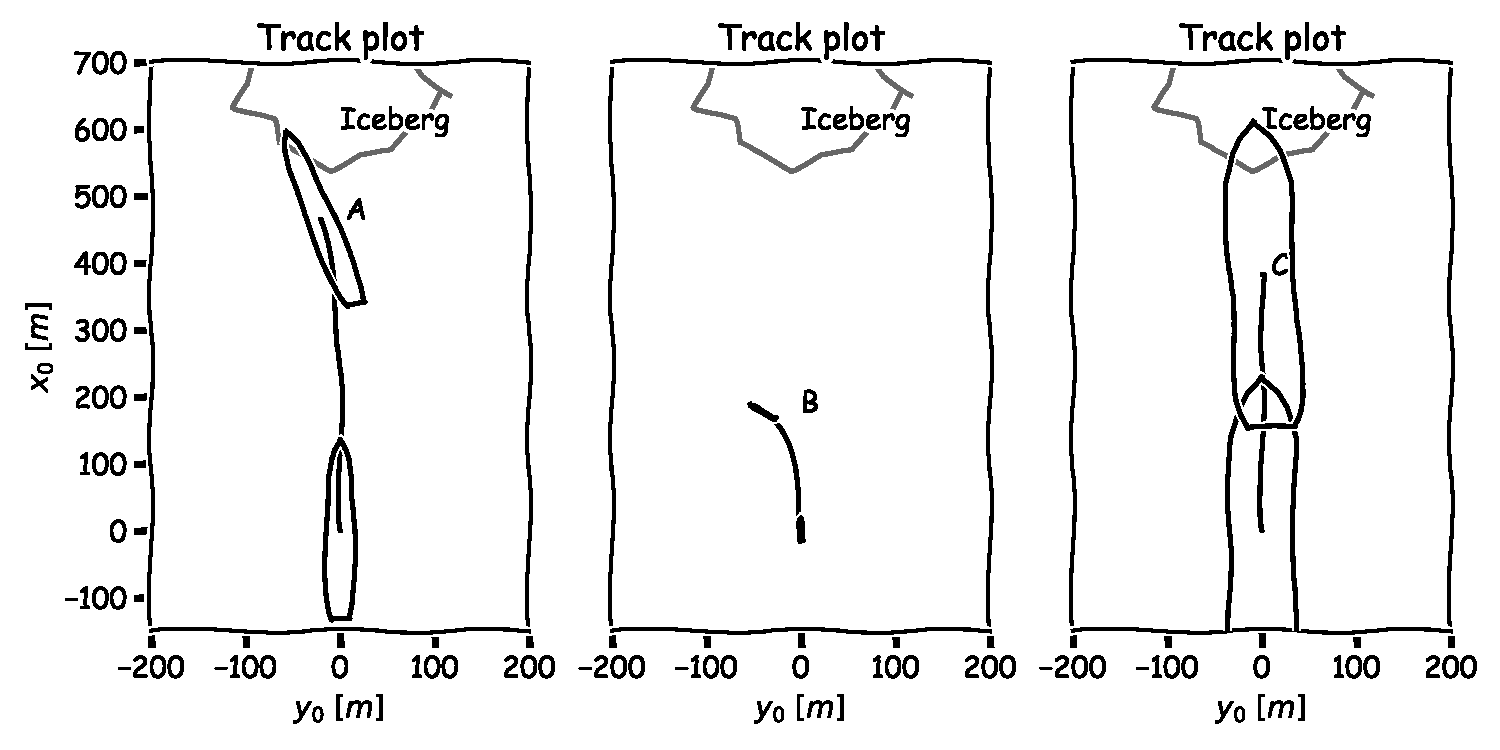
\includegraphics[width=3cm]{kappa/images/strip_1.pdf}
           \end{subfigure}
           
       \end{figure}
       
       
       };

  % Title
  \node [inner sep=0pt,anchor=south west, text width=17cm]  at
    ($ (current page.north west) + (1.8cm, -22.5cm) $)
     {
       \begin{spacing}{2}
         \textnohyphenation{\Huge \bfseries \textls*[40]{\thesistitle}}
        \end{spacing}
     };

  % Name
  \node [inner sep=0pt,anchor=north west, text width=16cm]  at
    ($ (current page.north west) + (1.8cm, -23.5cm) $)
     {\LARGE \textsc{\textls*[80]{\MakeUppercase{\thesisauthor}}}};

  % University
  \node [inner sep=0pt,anchor=north west, text width=16cm]  at
    ($ (current page.north west) + (1.8cm, -25.5cm) $)
     {
     \begin{spacing}{1.05}
     \textit{\large{Department of \thesisdepartment}}
     \par \vspace{0.15cm} \noindent
     \small \textsc{\textls*[80]{CHALMERS UNIVERSITY OF TECHNOLOGY}}
     \par \vspace{0.03cm} \noindent
     \large{Gothenburg, Sweden \thesisyear}
     \end{spacing}
   };

\end{tikzpicture}

\cleardoublepage  % advance two pages

\setcounter{page}{1}  % restart page numbering

\pagenumbering{roman}


\frontmatter                  % roman page numbers

{
\parindent 0 pt
\centering
\thispagestyle{empty}         % no page numbers here


\begin{normalsize}{\uppercase Thesis for the degree of 
\ifthenelse{\equal{\thesistype}{PhD}}{Doctor of Philosophy}{Licentiate of Engineering}}
\end{normalsize}

\vspace{3 cm}

{\large \textbf{\thesistitle} \par}
\vskip 1pc
{\large \thesissubtitle}
\vspace{1.5 cm}
\vspace{-10pt}

{\normalsize \MakeUppercase{\thesisauthor} \par}

\vspace{5 cm}


\includegraphics[width=35mm]{frontmatter/standard-images/chalmers_logo}
\vfill
\vspace{0.5 cm}

Department of \thesisdepartment \\
{\scshape CHALMERS UNIVERSITY OF TECHNOLOGY} \\
Gothenburg, Sweden \thesisyear

\newpage
}


\vspace*{50 pt}
{
  \thispagestyle{empty}         % no page numbers here

  \parindent 0 pt

  \thesistitle

  \thesissubtitle

  \textsc{\thesisauthor}

  \thesisisbn

  \vskip 1pc

  \copyright\enskip \textsc{\thesisauthor, \thesisyear.}

  \vskip 1pc

  \ifthenelse{\equal{\thesistype}{PhD}}{Doktorsavhandlingar}{Licentiatavhandlingar}
   vid Chalmers tekniska högskola

  \ifthenelse{\equal{\thesistype}{PhD}}{%
    Ny serie nr \thesisnumber%
  }{%
    Technical report No. \thesisnumber%
  }

  \thesisissn

  \vskip 1pc

  Department of \thesisdepartment

  Chalmers University of Technology

  SE--412 96 Göteborg, Sweden

  Telephone\enskip+ 46 (0) 31 -- 772 1000

  \vfill

  \thesiscoverdescription

  \vskip 2pc

  Typeset by the author using \LaTeX.

  \vskip 1pc

  Printed by Chalmers Reproservice

  Göteborg, Sweden \thesisyear
}

\clearpage


%\thispagestyle{empty}         % no page numbers here
\vspace*{10 pc}
\hfill{\it to my family}
\vfill
\clearpage


%==============================================================
% Abstract
%==============================================================
% Add abstract to the ToC
\cleardoublepage              % advance the pages
\pagenumbering{roman}
\phantomsection               % put pdf anchor
\addcontentsline{toc}{chapter}{Abstract}  % add toc line with target at the last anchor
\noindent\textbf{\thesistitle}\\

\noindent \MakeUppercase{\thesisauthor}\\
\noindent Chalmers University of Technology\\
\noindent \thesisdepartment\\
\section*{Abstract}
%\vspace*{-1cm}                % More space for abstract text

% -- Importance, background/motivation
It is common today that operational data is recorded onboard ships within the Internet of Ships (IoS) paradigm. This enables the possibility to build ship digital twins as digital copies of the real ships. Predicting the ship's motions with ship dynamics could be an important sub-component of these ship digital twins. A model for the ship's dynamics can be identified based on observations of the ship's motions. 
The identified model will have model uncertainty due to imperfections and idealizations made in physical model formulations as well as uncertainty from errors in the measurement data, which can be very pronounced when using full scale operational data. It is easier to develop accurate models with low model uncertainty using data obtained in a controlled laboratory environment where the measurement errors are much lower, especially in calm water conditions. The prediction model should be able to describe scenarios that a ship has never encountered before, which is possible if much of the underlying physics has been identified. Grey-box modelling is a technique which combines operational data with physical principles to achieve this. 
 
The objective of this thesis is to 
% -- Objective/scope
\noindent \objective 

% -- Method, developed method, setting
A model development procedure is proposed to handle the model uncertainty through the selection of candidate models based on a hold-out evaluation procedure. The measurement noise is handled by an iterative preprocessor, which uses an extended Kalman filter (EKF) and a Rauch Tung Striebel (RTS) smoother that uses an initially estimated predictor model from semi-empirical formulas.

% -- Results example
It is demonstrated that the ship's roll motion with high accuracy can be described using a quadratic damping model. For the more complex manoeuvring models, multicollinearity is a large problem where the appropriate complexity needs to be selected with the bias-variance trade-off between underfitting or overfitting the data. 
Hold-out turning circle tests were predicted with high accuracy for the wPCC and KVLCC2 test case ships with models from the proposed development procedure and parameter estimation method.

% -- Conclusion 
The proposed methods can produce prediction models with high generalization given that a suitable model structure has been selected from the candidate models and an appropriate split in the hold-out evaluation of the model development process has been applied. 

\vspace{0.3cm}
\noindent\textbf{Keywords:} Extended Kalman filter, Inverse dynamics, Multicollinearity, RTS smoother, Ship digital twin, Ship manoeuvring, System identification
\cleardoublepage


\phantomsection               % put pdf anchor
\addcontentsline{toc}{chapter}{Acknowledgments}  % add toc line with target at the last anchor
\section*{Preface}
This thesis presents research performed since February 2020 at the Division of Marine Technology, Department of Mechanics and Marine Sciences at Chalmers University of Technology and SSPA Sweden AB (\href{www.sspa.se}{www.sspa.se}). Financial support for this research was provided by the DEMOPS project (Development of Methods for Operational Performance of Ships) funded by Swedish Transport Administration (project: FP4 2020) and D2E2F project (Data Driven Energy Efficiency of Ships) funded by Swedish Energy Agency (project: 49301-1).

I had unsuccessfully been applying for funding for PhD studies for a couple of years when Professor Wengang Mao contacting me three years ago with the offer to become a PhD student. I will always be very grateful for this offer and I'm sure that I would otherwise be still searching for funding or given up by now. Wengang has also been my main supervisor during my studies and a guide to the academic research and a tutor in statistical and machine learning methods.  

This gratitude also goes to my examiner and co-supervisor, Professor Jonas W Ringsberg,
head of the Division of Marine Technology. I have enjoyed our discussions about research methodology and how to organize a paper in academic writing, where his detailed proof reading has also been a great asset.

I also want to thank SSPA Sweden AB for allowing me to be an industrial PhD student within my current employment. Special thanks to Dr. Christian Finnsgård head of the Research Department at SSPA, for his support and good advice throughout the project. I also want to mention all personnel at SSPA who have been involved in creating the model test results, building the ship models, and conducting the experiments.

\vskip 2pc

\noindent \thesisauthor

\noindent \thesiscity, October\  2022  % Since dedication is written a month or more before the actual thesis date, \thesismonth and \thesisyear is not used here.


% add Contents to PDF bookmarks, but do not add it to the 'printed' Contents
\cleardoublepage
\phantomsection
% \pdfbookmark[level]{text-to-display-in-outline}{unique-pdf-anchor-name}, chapter is level 0
\pdfbookmark[0]{Contents}{Contents}
\tableofcontents

\cleardoublepage              % advance the pages
\phantomsection               % put pdf anchor
\addcontentsline{toc}{chapter}{List of publications}  % add toc line with target at the last anchor
\chapter*{List of publications}
% This page is hand-made. I could not make Biblatex to output the papers the way I wanted.

%\begin{refsection}

This thesis is based on the following appended papers:

\begin{description}
% Biblatex \fullcite{Voronov2011} would work, but it uses maxcitenames, not maxbibnames, and there is no obvious way to change maxbibnames locally and change it back afterwards.
\item[Paper~\ref{pap:rolldamping}.]
\fullcite{alexandersson_analysis_2021}

%\item[Paper~\ref{pap:motions}.] 
%\fullcite{alexandersson_prediction_2021}

\item[Paper~\ref{pap:daiyong}.] 
\fullcite{alexandersson_comparison_2022}

\item[Paper~\ref{pap:pit}.] 
\fullcite{alexandersson_system_nodate}
\\
To be submitted to Ocean Engineering

\end{description}

\vspace{1cm}

\noindent Other relevant publications co-authored by Martin Alexandersson:
\begin{description}
\normalsize
\newcommand{\ME}{{\bfseries Martin Alexandersson}}

\item
Alexandersson, M., 2009. A STUDY OF METHODS TO PREDICT ADDED RESISTANCE IN WAVES. https://doi.org/10.13140/RG.2.2.18796.69767

\item
Alexandersson, M., Korkmaz, K., Mazza, G., 2017. Virtual Captive Tests with a destroyer hull form.

\item
Alexandersson, M., Kjellberg, M., Mao, W., Ringsberg, J., 2021. Prediction of roll motion using fully nonlinear potential flow and Ikeda’s method.


\end{description}

%\end{refsection}

\addcontentsline{toc}{chapter}{Nomenclature}  % add toc line with target at the 
%\mbox{}
\makenomenclature
\nomenclature{$\displaystyle OG$}{vertical distance into water from still water to centre of gravity\nomunit{m}}
\nomenclature{$\displaystyle A_{0}$}{mid ship area coefficient}
\nomenclature{$\displaystyle BK_{B}$}{bilge keel height\nomunit{m}}
\nomenclature{$\displaystyle BK_{L}$}{bilge keel length\nomunit{m}}
\nomenclature{$\displaystyle \phi_{a}$}{initial roll amplitude\nomunit{rad}}
\nomenclature{$\displaystyle A_{44}$}{total mass moment of inertia\nomunit{kg\cdot m^2}}
\nomenclature{$\displaystyle B_{1}$}{linear damping coefficient\nomunit{Nm/(rad/s)}}
\nomenclature{$\displaystyle B_{2}$}{quadratic damping coefficient\nomunit{Nm/(rad/s^2}}
\nomenclature{$\displaystyle B_{3}$}{cubic damping coefficient\nomunit{Nm/(rad/s)^3}}
\nomenclature{$\displaystyle B_{E}$}{eddy roll damping\nomunit{Nm/(rad/s)}}
\nomenclature{$\displaystyle B_{F}$}{friction roll damping\nomunit{Nm/(rad/s)}}
\nomenclature{$\displaystyle B_{L}$}{hull lift roll damping\nomunit{Nm/(rad/s)}}
\nomenclature{$\displaystyle B_{W}$}{wave roll damping\nomunit{Nm/(rad/s)}}
\nomenclature{$\displaystyle B_{BK}$}{bilge keel roll damping\nomunit{Nm/(rad/s)}}
\nomenclature{$\displaystyle C_{1}$}{linear stiffness coefficient\nomunit{Nm/rad}}
\nomenclature{$\displaystyle C_{3}$}{stiffness coefficient\nomunit{Nm/rad^3}}
\nomenclature{$\displaystyle C_{5}$}{stiffness coefficient\nomunit{Nm/rad^5}}
\nomenclature{$\displaystyle L$}{ship perpendicular length\nomunit{m}}
\nomenclature{$\displaystyle T$}{mean draught\nomunit{m}}
\nomenclature{$\displaystyle V$}{ship speed\nomunit{m/s}}
\nomenclature{$\displaystyle beam$}{ship beam\nomunit{m}}
\nomenclature{$\displaystyle \omega_{0}$}{natural angular velocity\nomunit{rad/s}}
\nomenclature{$\displaystyle t$}{time\nomunit{s}}
\nomenclature{$\displaystyle m$}{ship mass\nomunit{kg}}
\nomenclature{$\displaystyle \bigtriangledown$}{ship displacement\nomunit{m^3}}
\nomenclature{$\displaystyle \phi$}{ship roll angle\nomunit{rad}}
\nomenclature{$\displaystyle x_0$}{ship global position\nomunit{m}}
\nomenclature{$\displaystyle x_G$}{ship longitudinal centre of gravity\nomunit{m}}
\nomenclature{$\displaystyle GM$}{ship metacentric height \nomunit{m}}
\nomenclature{$\displaystyle g$}{gravity \nomunit{kg\cdot m/s^2}}
\nomenclature{$\displaystyle y_o$}{ship global position\nomunit{m}}
\nomenclature{$\displaystyle \Psi$}{ship heading \nomunit{rad}}
\nomenclature{$\displaystyle \beta$}{ship drift angle \nomunit{rad}}
\nomenclature{$\displaystyle \rho$}{water density \nomunit{kg/m^3}}
\nomenclature{$\displaystyle D$}{propeller diameter \nomunit{m}}
\nomenclature{$\displaystyle n$}{propeller speed \nomunit{rad/s}}
\nomenclature{$\displaystyle J$}{propeller advance ratio}
\nomenclature{$\displaystyle w_p$}{propeller wake fraction}
\nomenclature{$\displaystyle w_{p0}$}{taylor wake fraction}
\nomenclature{$\displaystyle x_p$}{propeller longitudinal position \nomunit{m}}
\nomenclature{$\displaystyle X$}{ship force in longitudinal direction \nomunit{N}}
\nomenclature{$\displaystyle Y$}{ship force in transverse direction \nomunit{N}}
\nomenclature{$\displaystyle N$}{ship yawing moment \nomunit{Nm}}
\nomenclature{$\displaystyle u$}{surge velocity\nomunit{m/s}}
\nomenclature{$\displaystyle v$}{sway velocity\nomunit{m/s}}
\nomenclature{$\displaystyle r$}{yaw rate\nomunit{rad/s}}
\nomenclature{$\displaystyle I_z$}{ship yaw moment of inertia\nomunit{kg\cdot m^2}}
\nomenclature{$\displaystyle \textbf{w}$}{process noise}
\nomenclature{$\displaystyle \textbf{c}$}{control signal}
\nomenclature{$\displaystyle \delta$}{rudder angle \nomunit{rad}}
\nomenclature{$\displaystyle \delta$}{rudder angle \nomunit{rad}}
\printnomenclature

\cleardoublepage              % advance the pages
\phantomsection               % put pdf anchor
\addcontentsline{toc}{chapter}{List of acronyms}  % add toc line with target at the last anchor
\chapter*{List of acronyms}
% To find all three-letter acronyms in file kappa/body.tex that are outside of comments: 
% grep -o "[^%]*" kappa/body.tex | grep -o "\b[A-Z][A-Z][A-Z]\b" | sort | uniq

\begin{tabular}{ l c l }
CFD & -- & Computational Fluid Dynamics\\
DOF & -- & Degree Of Freedom\\
FFT & -- & Fast Fourier Transform\\
ODE & -- & Ordinary Differential Equation\\
OLS & -- & Ordinary Least Squares\\
PIT & -- & Parameter Identification Technique\\
SI  & -- & Simplified Ikeda\\
VMM & -- & Vessel Manoeuvring Model\\

\end{tabular}




\mainmatter                   % normal arabic page numbers
%\part{Introductory chapters}
\pagenumbering{arabic}
% Headers, footers
\fancyfoot{}                  % clean all
\fancyhead[RE]{\textit{\nouppercase{\rightmark}}}
\fancyhead[RO]{\thepage}
\fancyhead[LE]{\thepage}
\fancyhead[LO]{\textit{\nouppercase{\leftmark}}}

%  \begin{refsection}

%!TEX root = ../main.tex

%%%%%%%%%%%%%%%%%%%%%%%%%%%%%%%
%%%%%%%%%%%%%%%%%%%%%%%%%%%%%%%
\chapter{Introduction}
%%%%%%%%%%%%%%%%%%%%%%%%%%%%%%%
The background of modelling the Ship Digital Twin (SDT) with white-, black- or grey-box models is first introduced in this chapter followed by a brief literature review. The motivation and objective of this research is then stated followed by assumptions and limitations. The chapter ends with an outline of the whole thesis.

\section{Background}
Shipbuilding 4.0, at the principles of the Industry 4.0, will transform the design, manufacturing, operation, shipping, services, production systems, maintenance and value chains in all aspects of the shipbuilding 
industry \cite{stanic_toward_2018}.
The emergence of Internet-of-Things (IoT) has led to the introduction of the Internet-of-Ships (IoS) paradigm. \begin{quote} IoS is the interconnecting of sensing objects, such as ships, crews, cargoes, onboard equipments, waterway environment, waterway facilities, shore-based facilities, and other navigation elements, which are embedded with a variety of sensor and heterogeneous network technologies to enable these objects to collect and exchange data \cite{liu_internet_2016-1}.\end{quote}
Safety enhancements, route planning and optimization, energy efficiency, automatic berthing and autonomous shipping are some of the emerging applications for IoS \cite{aslam_internet_2020}.
A SDT as a digital copy of a real ship, is one approach to achieve this \cite{chen_review_2021}. 
SDTs are data-driven in contrast to the related term Virtual Prototyping (VP), which is instead model based \cite{major_framework_2021}. A SDT is generally a model for an existing ship from where data can be collected and the VPs are generally prototypes for future ships, where no operational data is yet available.
In VP, white-box models are used. Either black-box or grey-box models are used in the SDTs. 

\begin{itemize}
    \item White-box modeling \\
    involves applying physical principles, so that no observed data is required, for instance Computational Fluid Dynamics (CFD). Semi-empirical models where unknown physical constants have been derived from historical experiments, can also be considered as white-box models \cite{leifsson_grey-box_2008}.  

    \item Black-box modeling \\
    means that parameters do not have physical significance but where the objectives is to find a good model that fits the observed data \cite{lindskog_tools_1995}.
    
    \item Grey-box modeling \\
    is a combination of white-box and black-box modeling methods, so that both a physical model and data is used. This concept is also referred as semi-physical modeling, hybrid modeling or semi-mechanistic modeling in the literature \cite{leifsson_grey-box_2008}. 
\end{itemize}

\noindent In a grey box model the white and black parts can be combined in several ways using either a serial or parallel approach \cite{leifsson_grey-box_2008} as seen in Fig.\ref{fig:greycombinations}. 

\begin{figure}[H]
    \centering
    \begin{subfigure}[b]{0.3\textwidth}
    \centering
    \begin{tikzpicture}[node distance=2cm]
    \node (white-box) [white-box] {White-box};
    \node (black-box) [black-box, right of=white-box, xshift=2cm] {Black-box};
    \draw [arrow] (white-box) -- (black-box);
    \end{tikzpicture}
    \caption{Serial grey-box}
    \label{fig:serial1}
    \end{subfigure}

    
    \begin{subfigure}[b]{0.3\textwidth}
    \centering
    \begin{tikzpicture}[node distance=2cm]
    \node (black-box) [black-box] {Black-box};
    \node (white-box) [white-box, right of=black-box, xshift=2cm] {White-box};
    \draw [arrow] (black-box) -- (white-box);
    \end{tikzpicture}
    \caption{Serial grey-box}
    \label{fig:serial2}
    \end{subfigure}

    \begin{subfigure}[b]{0.3\textwidth}
    \centering
    \begin{tikzpicture}[node distance=2cm]
    \node (black-box) [black-box] {Black-box};
    \node (white-box) [white-box, below of=black-box] {White-box};
    \node (join) [process, right of=black-box, xshift=2cm, yshift=-1cm] {join};
    \draw [arrow] (black-box) -- (join);
    \draw [arrow] (white-box) -- (join);
    \end{tikzpicture}
    \caption{Parallel grey-box}
    \label{fig:parallel}
    \end{subfigure}
    \caption{Several ways to combine white- and black-box models in grey box models.}
    \label{fig:greycombinations}
\end{figure}

\noindent The black-box modeling is entirely data driven, which means that no prior understanding of the system generating the data is needed and is therefore an attractive option for the SDT modelling. The black-box modeling may however give infeasible models outside the domain covered by the available data \cite{nielsen_machine_2022}. The white-box modeling does not have this problem, but does on the other hand require a full understanding of the system, which may be possible for special cases, but in general not possible for the complex scenario of a ship operating at sea. In the deep sea: wind, waves and current will add complexity. In coastal areas water depth and bank-effects will also add complexity \cite{nielsen_machine_2022}. 
\noindent Grey-box modelling is an attempt to bridge these problems, to either mitigate the white-box modelling error or the black-box extrapolation error.

Ship dynamics is a branch of ship hydrodynamics which concerns the ship forces and motions when the ship is allowed to move and rotate in all directions. Seakeeping and Manoeuvring are the two major sub fields, where Seakeeping studies the  behaviour of a ship in a seaway, under the influence of the external waves, currents and winds. Calm water conditions, lacking the external waves, are further assumed in Manoeuvring, which can either be thought of as an idealized simplification case of Seakeeping or actual conditions in sheltered environments. This thesis concerns rigid body ship dynamics in calm waters. The rigid body assumption simplifies the ship as a stiff body that does not transform under the act of forces. In this thesis, the rigid body ship dynamics is studied with the aim to develop better SDTs with grey-box modeling.

\section{Literature review}
SDT has a a positive trend in the number of publications during the recent years (2018-2021)  \cite{assani_ships_2022}. Most of the papers concerns ship equipment such as electric power systems, propulsion system, ship hull structure and marine diesel engines \cite{assani_ships_2022}. Only a minor part of the SDT applications handle ship trajectory, speed and fuel consumption \cite{assani_ships_2022}.   
Even though SDT is not explicitly mentioned, there are a lot of papers published about methods that can be used as SDTs. \cite{lang_comparison_2022} predicted the propulsion power for a chemical tanker for three test case voyages with high accuracy, using ML black-box modeling. The manoeuvres where however excluded. In another paper \cite{nielsen_machine_2022} used grey-box modelling for manoeuvring prediction of a ferry where a deep learning model (black-box) captures the residues between first-principles model (white-box) and observed data. These are very promising works that also show that there is still a lot to be done withing the field. 
A lot of research concerns the system identification of the ship's manoeuvring dynamics where a majority of the publications use simulated data as used in 
\cite{shi_identification_2009}, \cite{perera_system_2015}, \cite{zhu_parameter_2017} and \cite{wang_parameter_2021}. Some of the publications, for instance \cite{luo_parameter_2016} and \cite{he_nonparametric_2022} use data from physical model tests, where the measurement noise and the model uncertainty increases the complexity. 


%"Critic" to what has been done before
\section{Motivation and objective}
\label{sec:motivation}
% Motivation:
Huge amounts of data concerning ships' operation is collected daily around the oceans. We are still figuring out ways to make use of it. Models specialized in predicting specific aspects of the ship's operation, such as the fuel consumption, can be developed as black-box models with the latest technologies within Machine Learning (ML). It is in the author's belief that grey-box models, also incorporating physical relations, could give better prediction models to improve the SDTs. Introducing some aspects of ship dynamics into the model, gives a deeper understanding of the forces and motions of the ship, which can improve the accuracy of the SDTs to be used in the IoS applications. This approach will be explored in this thesis for the ship rigid body dynamics in calm waters.

Full scale operational data from ships at sea has a lot of noise and large uncertainties, due to the sea environment. Developing SDTs for this data is a great challenge. It is especially hard to know when the model is correct and when it is not. Instead, using data from a controlled laboratory environment, offers data from a similar environment, but with less noise and uncertainties. 
Model test data is therefore used in this thesis to develop SDT grey-box models of the ship rigid body dynamics. The hypothesis is that a SDT model that works in the lab, will also have potential to work at the sea. Or at least false models can be ruled out, since SDT models that do not work in the lab, will most likely not work at sea either. 

% Objective: 
\bigskip
\noindent Starting with reduced complexity and then gradually increasing the complexity has been a general approach to formulate the research objectives for this thesis:   


\subsubsection*{SDT for roll motion}
The first objective of the thesis is therefore to develop a SDT for the calm water ship rigid body dynamics in the roll degree of freedom, based on model test data.

\subsubsection*{SDT for manoeuvring}
The second objective is to increase the complexity by adding the surge, sway and yaw degrees of freedoms, addressing the manoeuvring problem.

\subsubsection*{SDT generalization}
The SDT must be able to make predictions outside the domain covered by the available data, in order to be of practical use in IoS applications. This addresses the generalization of the SDTs.

\section{Assumptions and limitations}
%Calm waters...
Calm water condition is a simplification of the real sea condition that a ship encounters. This condition assumes that the influences from encountering wind, waves and currents are neglected. These assumptions simplifies the system identification, by reducing the degrees of freedoms to: surge, sway, yaw and roll. Also note that all result are not necessarily directly transferable to full scale when model scale data is used, considering potential scale effects. 

\section{Outline of the thesis}
Chapter \ref{ch:models} presents the models for ship rigid body dynamics used in this thesis. The models for roll motion is introduced in Section \ref{sec:roll} and the manoeuvring motion models are introduced in Section \ref{sec:VMM}. These models represent the physical principles and thereby the white-box part of the developed grey-box models.
Parameter Identification Techniques (PITs), representing the black-box part, are used to regress the parameters of the white-box models. The PITs are introduced in Chapter \ref{ch:methods} for the roll motion and the manoeuvring motion in Section \ref{sec:PIT_roll} and Section \ref{sec:PIT_VMM}. 
A short summary of the appended papers, including research activities and a selection of the important results is presented in chapter \ref{ch:results}, followed by the conclusions in chapter \ref{ch:conclusions} and plans for future work in chapter \ref{ch:future_work}.
%%%%%%%%%%%%%%%%%%%%%%%%%%%%%%%
%%%%%%%%%%%%%%%%%%%%%%%%%%%%%%%
\chapter{Ship rigid body dynamics models}
\label{ch:models}
%%%%%%%%%%%%%%%%%%%%%%%%%%%%%%%

The ship's dynamics comprises the forces and motions in the six degrees of freedoms (6DOF): surge, sway, heave, roll, pitch and yaw. Heave and pitch motions are often neglected in calm water conditions, so that a four degrees of freedom (4DOF) model is sufficient to express the ship's dynamics. Physically parameterized models for roll and the Vessel Manoeuvring Model (VMM) for the remaining DOFs are presented in section \ref{sec:roll} and section \ref{sec:VMM}. How the parameters in these models can be identified is presented in \ref{sec:PIT_roll}.

\section{Roll motion} \label{sec:roll}

The roll motion on a straight course in calm water with no external forces can be expressed with Eq.\ref{eq:roll_decay_equation_general_himeno} \cite{himeno_prediction_1981},
\begin{equation} \label{eq:roll_decay_equation_general_himeno}
A_{44} \ddot{\phi} + \operatorname{B_{44}}\left(\dot{\phi}\right) + \operatorname{C_{44}}\left(\phi\right) = 0
\end{equation}


\noindent where $B_{44}\left(\dot{\phi}\right)$ can be expressed as expansion series:  
$ B_{44}\left(\dot{\phi}\right) = B_1\cdot\dot{\phi} + B_2\cdot\dot{\phi}\left|\dot{\phi}\right| + B_3\cdot\dot{\phi}^3 + ... + B_n\cdot\dot{\phi}^n$. Most often, the so-called ``linear model'' (Eq.\ref{eq:roll_decay_equation_himeno_linear}), ``quadratic model'' (Eq.\ref{eq:roll_decay_equation_himeno_quadratic_b}) and ``cubic model'' (Eq.\ref{eq:roll_decay_equation_cubic}) are used to represent $B_{44}(\dot{\phi})$ in by truncating the series to keep only linear, quadratic and cubic terms,

\begin{equation} \label{eq:roll_decay_equation_himeno_linear}
A_{44} \ddot{\phi} + B_{1} \dot{\phi} + C_{1} \phi = 0
\end{equation}

\begin{equation} \label{eq:roll_decay_equation_himeno_quadratic_b}
A_{44} \ddot{\phi} + C_{1} \phi + \left(B_{1} + B_{2} \left|{\dot{\phi}}\right|\right) \dot{\phi} = 0
\end{equation}

\begin{equation} \label{eq:roll_decay_equation_cubic}
A_{44} \ddot{\phi} + \left(B_{1} + B_{2} \left|{\dot{\phi}}\right| + B_{3} \dot{\phi}^{2}\right) \dot{\phi} + \left(C_{1} + C_{3} \phi^{2} + C_{5} \phi^{4}\right) \phi = 0
\end{equation}


\section{Vessel Manoeuvring Models} \label{sec:manoeuvring model}
\label{\detokenize{02.01_manoeuvring models:vessel-manoeuvring-models}}\label{\detokenize{02.01_manoeuvring models:vmm}}\label{\detokenize{02.01_manoeuvring models::doc}}
Ship manoeuvring is a simplified case of seakeeping. The encountering waves have been removed, assuming calm water conditions. The manoeuvring motions have low frequencies so that added masses and other hydrodynamic derivatives can be assumed as constants  \cite{fossen_handbook_2021}. Three manoeuvring models are used in this thesis: 
\begin{itemize}
    \item Linear (LVMM) \cite{matusiak_dynamics_2017}
    \item Abkowitz (AVMM), \cite{abkowitz_ship_1964}
    \item Modified Abkowitz (MAVMM), which is proposed in Paper \ref{pap:pit}
\end{itemize}

\noindent\autoref{\detokenize{02.01_manoeuvring models:coordinate-system}} shows the reference frames used in the manoeuvring models where \(x_0\) and \(y_0\) and heading \(\Psi\) are the global position and orientation of a ship fix reference frame \(O(x,y,z)\) (or rather \(O(x,y)\) when heave is excluded) with origin at midship. \(u\), \(v\), \(r\), \(X\), \(Y\) and \(N\) are velocities and forces in the ship fix reference frame.



\begin{figure}[H]
    \centering
    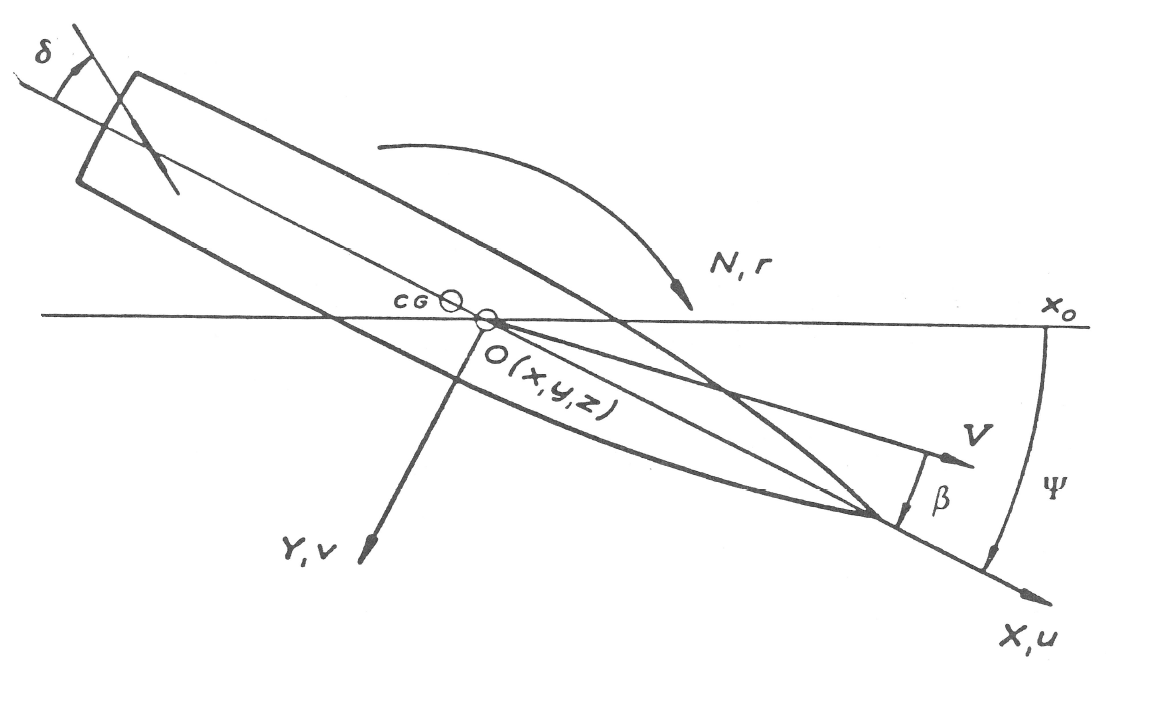
\includegraphics[width=0.8\textwidth]{kappa/images/coordinate_system.PNG}
    \caption{Reference frames.}
    \label{\detokenize{02.01_manoeuvring models:coordinate-system}}
\end{figure}

The manoeuvring equation can be described as \cite{fossen_handbook_2021},
\begin{equation}\label{equation:02.01_manoeuvring models:eqqsystem}
\begin{split}\displaystyle \left[\begin{matrix}- X_{\dot{u}} + m & 0 & 0\\0 & - Y_{\dot{v}} + m & - Y_{\dot{r}} + m x_{G}\\0 & - N_{\dot{v}} + m x_{G} & I_{z} - N_{\dot{r}}\end{matrix}\right] \left[\begin{matrix}\dot{u}\\\dot{v}\\\dot{r}\end{matrix}\right] = \left[\begin{matrix}m r^{2} x_{G} + m r v + \operatorname{X_{D}}{\left(u,v,r,\delta,thrust \right)}\\- m r u + \operatorname{Y_{D}}{\left(u,v,r,\delta,thrust \right)}\\- m r u x_{G} + \operatorname{N_{D}}{\left(u,v,r,\delta,thrust \right)}\end{matrix}\right]\end{split}
\end{equation}

\noindent where the first matrix describes the inertia of the ship in the surge, sway and yaw directions. The inertia in air is represented by the mass $m$ and moment of inertia $I_z$. The added mass in water is represented by: $X_{\dot{u}}$, $Y_{\dot{v}}$, $Y_{\dot{r}}$, $N_{\dot{v}}$ and $N_{\dot{r}}$. The hydrodynamic forces from the ship hull and rudder are desribed in the functions $X_D()$, $Y_D()$ and $N_D()$. The accelerations ($\dot{u}$, $\dot{v}$ and $\dot{r}$) can be solved from this equation,
\begin{equation}\label{equation:02.01_manoeuvring models:eqacc}
\begin{split}\displaystyle \dot{\nu} = \left[\begin{matrix}\dot{u}\\\dot{v}\\\dot{r}\end{matrix}\right] = \left[\begin{matrix}\frac{1}{- X_{\dot{u}} + m} & 0 & 0\\0 & - \frac{- I_{z} + N_{\dot{r}}}{S} & - \frac{- Y_{\dot{r}} + m x_{G}}{S}\\0 & - \frac{- N_{\dot{v}} + m x_{G}}{S} & - \frac{Y_{\dot{v}} - m}{S}\end{matrix}\right] \left[\begin{matrix}m r^{2} x_{G} + m r v + \operatorname{X_{D}}{\left(u,v,r,\delta,thrust \right)}\\- m r u + \operatorname{Y_{D}}{\left(u,v,r,\delta,thrust \right)}\\- m r u x_{G} + \operatorname{N_{D}}{\left(u,v,r,\delta,thrust \right)}\end{matrix}\right]\end{split}
\end{equation}
\sphinxAtStartPar
where \(S\) is a helper variable:
\begin{equation}\label{equation:02.01_manoeuvring models:eq_S}
\begin{split}\displaystyle S = - I_{z} Y_{\dot{v}} + I_{z} m + N_{\dot{r}} Y_{\dot{v}} - N_{\dot{r}} m - N_{\dot{v}} Y_{\dot{r}} + N_{\dot{v}} m x_{G} + Y_{\dot{r}} m x_{G} - m^{2} x_{G}^{2}\end{split}
\end{equation}
\sphinxAtStartPar

\noindent A state space model for manoeuvring can now be defined with six states:
\begin{equation}\label{equation:02.01_manoeuvring models:eq_x}
\begin{split}\displaystyle \mathbf{x} = \left[\begin{matrix}x_{0}\\y_{0}\\\Psi\\u\\v\\r\end{matrix}\right]\end{split}
\end{equation}
\noindent where $x_0$, $y_0$ and $\Psi$ are the global coordinates and heading of the ship and $u$, $v$ and $r$ are the velocities as seen in \autoref{\detokenize{02.01_manoeuvring models:coordinate-system}}.
The time derivative of this state \(\dot{\mathbf{x}}\) can be defined by a state transition \(f(\mathbf{x},\mathbf{c})\) using geometrical relations
how global coordinates \(x_0\), \(y_0\) and \(\Psi\) depend on \(u\), \(v\), and \(r\) viz.,
\begin{equation}\label{equation:02.01_manoeuvring models:eqf}
\begin{split}\displaystyle \dot{\mathbf{x}} = f(\mathbf{x},\mathbf{c}) + \mathbf{w}
                                          = \left[\begin{matrix}\dot{x_0}\\ \dot{y_0} \\ \dot{\Psi} \\\dot{u}\\\dot{v}\\\dot{r}\end{matrix}\right] + \mathbf{w}
                                          = \left[\begin{matrix}u \cos{\left(\Psi \right)} - v \sin{\left(\Psi \right)}\\u \sin{\left(\Psi \right)} + v \cos{\left(\Psi \right)}\\r\\\dot{u}\\\dot{v}\\\dot{r}\end{matrix}\right] + \mathbf{w}\end{split}
\end{equation}
\sphinxAtStartPar
where \(\mathbf{c}\) is control inputs (rudder angle \(\delta\) and thrust); the last three derivatives: \(\dot{u}\), \(\dot{v}\), \(\dot{r}\) are calculated with \autoref{equation:02.01_manoeuvring models:eqacc}.
\(\mathbf{w}\) is the process noise, i.e., the difference between the predicted state by the manoeuvring model and the true
state of the system. \(\mathbf{w}\) is unknown when the manoeuvring model is used for manoeuvre predictions and therefore normally
assumed to be zero, but it is an important factor when the manoeuvring model is used in the EKF (see \autoref{sec:datacleaning}).
The manoeuvring simulation can now be conducted by numerical integration of \autoref{equation:02.01_manoeuvring models:eqf}. The main difference between the manoeuvring model:s lies in how the hydrodynamic functions \(X_D(u,v,r,\delta,thrust)\), \(Y_D(u,v,r,\delta,thrust)\), \(N_D(u,v,r,\delta,thrust)\) are defined. These expressions are denoted in prime system ($X_D'$, $Y_D'$, $N_D'$) below for the various manoeuvring models: LVMM, AVMM and MAVMM.

{\normalfont \textbf{Linear vessel manoeuvring model (LVMM) \cite{matusiak_dynamics_2017}}}
\begin{equation}\label{equation:02.01_manoeuvring models:eqxlinear}
\begin{split}\begin{split}
\operatorname{X_{D}'}{\left(u',v',r',\delta\right)} = & X_{\delta} \delta + X_{r} r' + X_{u} u' + X_{v} v' 
\end{split}\end{split}
\end{equation}\begin{equation}\label{equation:02.01_manoeuvring models:eqylinear}
\begin{split}\begin{split}
\operatorname{Y_{D}'}{\left(u',v',r',\delta \right)} = & Y_{\delta} \delta + Y_{r} r' + Y_{u} u' + Y_{v} v' 
\end{split}\end{split}
\end{equation}\begin{equation}\label{equation:02.01_manoeuvring models:eqnlinear}
\begin{split}\begin{split}
\operatorname{N_{D}'}{\left(u',v',r',\delta \right)} = & N_{\delta} \delta + N_{r} r' + N_{u} u' + N_{v} v' 
\end{split}\end{split}
\end{equation}
\sphinxAtStartPar
{\normalfont \textbf{Abkowitz vessel manoeuvring model(AVMM) \cite{abkowitz_ship_1964}}}
\begin{equation}\label{equation:02.01_manoeuvring models:eqxabkowitz}
\begin{split}
\operatorname{X_{D}'}{\left(u',v',r',\delta,thrust' \right)} = & X_{\delta\delta} \delta^{2} + X_{r\delta} \delta r' + X_{rr} r'^{2} + X_{T} thrust' + X_{u\delta\delta} \delta^{2} u' \\ 
& + X_{ur\delta} \delta r' u' + X_{urr} r'^{2} u' + X_{uuu} u'^{3} + X_{uu} u'^{2} \\ 
& + X_{uv\delta} \delta u' v' + X_{uvr} r' u' v' + X_{uvv} u' v'^{2} \\
& + X_{u} u' + X_{v\delta} \delta v' + X_{vr} r' v' + X_{vv} v'^{2} 
\end{split}
\end{equation}

\begin{equation}\label{equation:02.01_manoeuvring models:eqyabkowitz}
\begin{split}\begin{split}
\operatorname{Y_{D}'}{\left(u',v',r',\delta,thrust' \right)} = & Y_{0uu} u'^{2} + Y_{0u} u' + Y_{0} + Y_{\delta\delta\delta} \delta^{3} + Y_{\delta} \delta + Y_{r\delta\delta} \delta^{2} r' + Y_{rr\delta} \delta r'^{2} \\ & + Y_{rrr} r'^{3} + Y_{r} r' + Y_{T\delta} \delta thrust' + Y_{T} thrust' + Y_{u\delta} \delta u' \\ & + Y_{ur} r' u' + Y_{uu\delta} \delta u'^{2} + Y_{uur} r' u'^{2} + Y_{uuv} u'^{2} v' + Y_{uv} u' v' \\ & + Y_{v\delta\delta} \delta^{2} v' + Y_{vr\delta} \delta r' v' + Y_{vrr} r'^{2} v' + Y_{vv\delta} \delta v'^{2} + Y_{vvr} r' v'^{2} \\ & + Y_{vvv} v'^{3} + Y_{v} v' 
\end{split}\end{split}
\end{equation}\begin{equation}\label{equation:02.01_manoeuvring models:eqnabkowitz}
\begin{split}\begin{split}
\operatorname{N_{D}'}{\left(u',v',r',\delta,thrust' \right)} = & N_{0uu} u'^{2} + N_{0u} u' + N_{0} + N_{\delta\delta\delta} \delta^{3} + N_{\delta} \delta + N_{r\delta\delta} \delta^{2} r' + N_{rr\delta} \delta r'^{2} \\ & + N_{rrr} r'^{3} + N_{r} r' + N_{T\delta} \delta thrust' + N_{T} thrust' + N_{u\delta} \delta u' \\ & + N_{ur} r' u' + N_{uu\delta} \delta u'^{2} + N_{uur} r' u'^{2} + N_{uuv} u'^{2} v' + N_{uv} u' v' \\ & + N_{v\delta\delta} \delta^{2} v' + N_{vr\delta} \delta r' v' + N_{vrr} r'^{2} v' + N_{vv\delta} \delta v'^{2} + N_{vvr} r' v'^{2} \\ & + N_{vvv} v'^{3} + N_{v} v' 
\end{split}\end{split}
\end{equation}
\sphinxAtStartPar
{\normalfont \textbf{Modified Abkowitz vessel manoeuvring model (MAVMM)}}
\newline
Only the most relevant coefficients in AVMM are included, as proposed in Paper \ref{pap:pit}.
\begin{equation}\label{equation:02.01_manoeuvring models:eqxmartinssimple}
\begin{split}\begin{split}
\operatorname{X_{D}'}{\left(u',v',r',\delta,thrust' \right)} = & X_{\delta\delta} \delta^{2} + X_{rr} r'^{2} + X_{T} thrust' + X_{uu} u'^{2} + X_{u} u' + X_{vr} r' v' 
\end{split}\end{split}
\end{equation}\begin{equation}\label{equation:02.01_manoeuvring models:eqymartinssimple}
\begin{split}\begin{split}
\operatorname{Y_{D}'}{\left(u',v',r',\delta,thrust' \right)} = & Y_{\delta} \delta + Y_{r} r' + Y_{T\delta} \delta thrust' + Y_{T} thrust' + Y_{ur} r' u' \\ & + Y_{u} u' + Y_{vv\delta} \delta v'^{2} + Y_{v} v' 
\end{split}\end{split}
\end{equation}\begin{equation}\label{equation:02.01_manoeuvring models:eqnmartinssimple}
\begin{split}\begin{split}
\operatorname{N_{D}'}{\left(u',v',r',\delta,thrust' \right)} = & N_{\delta} \delta + N_{r} r' + N_{T\delta} \delta thrust' + N_{T} thrust' + N_{ur} r' u' + N_{u} u' \\ & + N_{vv\delta} \delta v'^{2} + N_{v} v' 
\end{split}\end{split}
\end{equation}
\sphinxAtStartPar
The hydrodynamic functions above are expressed using nondimensional units with the prime system, denoted by the prime symbol (\('\)). The quantities are expressed in the prime system, using the denominators in Tab.\ref{tab:my_label}. For instance, surge linear velocity \(u\) can be expressed in the prime system as seen in \autoref{equation:02.01_manoeuvring models:eqprime} using the linear velocity denominator.
\begin{equation}\label{equation:02.01_manoeuvring models:eqprime}
\begin{split}\displaystyle u'=\frac{u}{V}\end{split}
\end{equation}
\sphinxAtStartPar
Equations can either be written in the prime or regular Standard Institute (SI) system. The hydrodynamic derivatives are always expressing forces in the prime system as function of state variables. The (\('\)) sign is therefore implicit and not written out as seen in \autoref{equation:02.01_manoeuvring models:eqderivativeprime}.
\begin{equation}\label{equation:02.01_manoeuvring models:eqderivativeprime}
\begin{split}\displaystyle Y_{\delta'}'=\frac{\partial Y_D'}{\partial \delta'} := Y_{\delta} \end{split}
\end{equation}
\sphinxAtStartPar
The exceptions are the added masses (\(X_{\dot{u}}\), \(Y_{\dot{v}}\), \(Y_{\dot{r}}\), \(N_{\dot{v}}\) and \(N_{\dot{r}}\)) which are expressed in both Prime system or the regular SI system where the (\('\)) sign is therefore
explicitly stated.
There is however a great benefit in expressing the hydrodynamic forces in the prime system. The forces are often nonlinear due to a quadratic relation to the flow velocity, as seen in \autoref{equation:02.01_manoeuvring models:eqquadraticsi}.
\begin{equation}\label{equation:02.01_manoeuvring models:eqquadraticsi}
\begin{split}\displaystyle Y_{D}=Y_{\delta} \cdot \delta \cdot \frac{L^2V^2\rho}{2}\end{split}
\end{equation}
which becomes linear when expressed in the prime system as seen in \autoref{equation:02.01_manoeuvring models:eqquadraticprime}.
\begin{equation}\label{equation:02.01_manoeuvring models:eqquadraticprime}
\begin{split}\displaystyle Y_{D}'=Y_{\delta} \cdot \delta'\end{split}
\end{equation}


\begin{table}[]
\caption{Prime system denominators.}
\label{tab:prime-system-denominators}
\centering
\label{tab:my_label}
\begin{tabular}{c c}
\toprule
Quantity &
Denominators
\\
\hline

angle
&

\(1\)
\\


angular
acceleration
&

\(\frac{V^{2}}{L^{2}}\)
\\


angular
velocity
&

\(\frac{V}{L}\)
\\


area
&

\(L^{2}\)
\\


density
&

\(\frac{\rho}{2}\)
\\


force
&

\(\frac{L^{2} V^{2} \rho}{2}\)
\\


frequency
&

\(\frac{V}{L}\)
\\


inertia
moment
&

\(\frac{L^{5} \rho}{2}\)
\\


length
&

\(L\)
\\


linear
acceleration
&

\(\frac{V^{2}}{L}\)
\\


linear
velocity
&

\(V\)
\\


mass
&

\(\frac{L^{3} \rho}{2}\)
\\


moment
&

\(\frac{L^{3} V^{2} \rho}{2}\)
\\


time
&

\(\frac{L}{V}\)
\\


volume
&

\(L^{3}\)
\\
\bottomrule

\end{tabular}


\end{table}

\subsection{The propeller model}
\label{\detokenize{02.10_propeller_model:the-propeller-model}}\label{\detokenize{02.10_propeller_model::doc}}

A propeller model is developed based on Manoeuvring Modeling Group (MMG) model \cite{yasukawa_introduction_2015-1} where the thrust is expressed as:
\begin{equation}\label{equation:02.10_propeller_model:eqT}
\begin{split}\displaystyle thrust = D^{4} K_{T} n^{2} \rho\end{split}
\end{equation}

and the thrust coefficient \(K_T\) is modelled as a second order polynomial:
\begin{equation}\label{equation:02.10_propeller_model:eqkt}
\begin{split}\displaystyle K_{T} = J^{2} k_{2} + J k_{1} + k_{0}\end{split}
\end{equation}

The advance ratio \(J\) is calculated as:
\begin{equation}\label{equation:02.10_propeller_model:eqJ}
\begin{split}\displaystyle J = \frac{u \left(1 - w_{p}\right)}{D n}\end{split}
\end{equation}

where \(D\) is propeller diameter, \(n\) is propeller speed and \(w_p\) is the wake fraction at an oblique inflow to the propeller from the drift angle and the yaw rate. A semi\sphinxhyphen{}empirical formula for \(w_p\) is provided in the MMG model. As an alternative, a simple polynomial is proposed in \autoref{equation:02.10_propeller_model:eqpropellermodel}.
\begin{equation}\label{equation:02.10_propeller_model:eqpropellermodel}
\begin{split}\displaystyle w_{p} = C_{1} \delta + C_{2} \delta^{2} + C_{3} \beta_{p}^{2} + C_{4} u + w_{p0}\end{split}
\end{equation}

\(w_p\) is modeled as a function of rudder angle \(\delta\), to include wake influence from the rudder and ship speed \(u\), to include a speed dependency. The influence from drift angle \(\beta\) and yaw rate \(r\) is expressed by \(\beta_p\) in \autoref{equation:02.10_propeller_model:eqbetap}.
\begin{equation}\label{equation:02.10_propeller_model:eqbetap}
\begin{split}\beta_p=\beta - \frac{r}{V} \cdot x_p \end{split}
\end{equation}

Where \(x_p\) is the propeller longitudinal position and \(w_{p0}\) is the regular Taylor wake fraction, applicable to straight ahead steaming with no rudder angle. Similar to the MMG propeller model, two sets of parameters \(C_1\)-\(C_4\) should be used in the propeller model depending on the sign of \(\beta_p\).
%%%%%%%%%%%%%%%%%%%%%%%%%%%%%%%
%%%%%%%%%%%%%%%%%%%%%%%%%%%%%%%
\chapter{Methods\label{ch:methods}}
%%%%%%%%%%%%%%%%%%%%%%%%%%%%%%%
The system identification of ship dynamics can be simplified into parameter identification if parameterized physical models can be assumed. Parameter Identification Techniques (PIT) for roll motion an manoeuvring is presented in \ref{sec:PIT_roll} and \ref{sec:PIT_VMM}. The system identification can be performed by selecting the best model from a collection of candidate models.

\section{Roll damping Parameter Identification} \label{sec:PIT_roll}
\noindent The PIT for roll motions can be applied to identify the roll damping parameters ($B_1$, $B_2$, $B_3$) and stiffness parameters ($C_1$, $C_3$, $C_5$) in the parameterized roll motion models in Eq.\ref{eq:roll_decay_equation_himeno_linear}, Eq.\ref{eq:roll_decay_equation_himeno_quadratic_b} and Eq.\ref{eq:roll_decay_equation_cubic}. These equations do not have unique solutions, considering that the whole equations can be multiplied by an arbitrary factor to obtain new valid solutions. The inertia is therefore excluded, to obtain unique solutions. This is achieved by normalizing the equations by the total roll inertia $A_{44}$ as seen in Eq.\ref{eq:roll_decay_nonedim_a44} for the linear model.

\begin{equation} \label{eq:roll_decay_nonedim_a44}
\ddot{\phi} + \frac{B_{1}}{A_{44}} \dot{\phi} + \frac{C_{1}}{A_{44}} \phi = 
\ddot{\phi} + B_{1A} \dot{\phi} + C_{1A} \phi = 0
\end{equation}

\noindent The normalized damping and stiffness parameters $B_{1A}$ and $C_{1A}$ identified by a PIT can be expressed in dimensional units by multiplication with the normalization factor $A_{44}$. If $A_{44}$ is not known before hand, it can be calculated using Eq.\ref{eq:A_44_eq} \cite{piehl_ship_2016}, assuming that the meta center height $GM$ is known.
\begin{equation} \label{eq:A_44_eq}
A_{44} = \frac{GM g m}{\omega_{0}^{2}}
\end{equation}


\noindent The frequency $\omega_0$ can be obtained with Fast Fourier Transform (FFT) of the roll signal. 
Two different PIT methods have been investigated: the ``derivation approach'', referred as PIT in \parencite{imo_1200_2006}, and the ``integration approach'' as used in \cite{soder_assessment_2019}. 

\subsection{Derivation approach}\label{sec:derivation_approach}
In the derivation approach Eq.\ref{eq:roll_decay_nonedim_a44} is treated as a linear regression problem, where the states ($\phi$, $\dot{\phi}$, $\ddot{\phi}$) are known and the parameters should be regressed. Only roll angle $\phi$ is known from the experimental data, which means that the velocity and acceleration $\dot{\phi}$, $\ddot{\phi}$ needs to be estimated. A least squares fit is applied on the roll motion equation to identify any parameter, including nonlinear or frequency parameter. 

\subsection{Integration approach}\label{sec:integration_approach}
In the integration approach, Eq.\ref{eq:roll_decay_nonedim_a44} is solved as an Ordinary Differential Equation (ODE) for many estimated sets of parameters until the solution converges. This method is very time consuming and convergence is not guaranteed.

\section{VMM Parameter Identification} \label{sec:PIT_VMM}
The proposed PIT for VMMs is summarized in Fig.\ref{fig:greyvmm}. In this procedure, a VMM is used to solve the reversed manoeuvring problem, such as predicting unknown forces from known manoeuvring model test data. The hydrodynamic derivatives in the VMM can be identified with regression of the force polynomials on forces predicted with inverse dynamics (see Section \ref{\detokenize{03.01_inverse_dynamics::doc}}).
The measurement noise needs to be removed if the regression of hydrodynamic derivatives in the VMM should work well. This is conducted by a Extended Kalman Filter (EKF) and Rauch Tung Striebel (RTS) smoother (see section \ref{sec:datacleaning}). The EKF requires an accurate VMM as the predictor.
Therefore the accurate VMM is both the input and output of the PIT. The system model VMM in the EKF is guessed to solve this dilemma. A linear VMM with hydrodynamic derivatives estimated with semi-empirical formulas is used as the initial guess. Once the regressed VMM has been obtained, the PIT can be rerun using the regressed VMM as the system model in the EKF, to obtain an even better VMM. This procedure, indicated by the dashed arrow in Fig.\ref{fig:greyvmm}, can be repeated several times for improved accuracy. Using semi-empirical formulas for the initially guessed VMM adds prior knowledge about the ship dynamics to the regression. An example with simulation results from the steps in the iterative EKF is shown in \hyperref[\detokenize{01.01_method:iterations}]{Fig.\@\ref{\detokenize{01.01_method:iterations}}}.
\newpage
\begin{figure}[H]
    
    \centering
    \begin{tikzpicture}[node distance=1.5cm]
    %\draw (0,0) rectangle (10,10); %create a bounding box to reserve space
    \node (data) [io] {Model test data};
    
    \node (EKF) [process, right of=data, xshift=3.0cm] {EFK + RTS};
    \node (predictor) [process, right of=EKF, xshift=2.0cm]{Predictor};
    \node (VMM) [io, right of=predictor, xshift=1.0cm] {VMM initial};
    
    \node (data_clean) [io, below of=EKF] {\(x,\dot{x},\ddot{x}, \delta, thrust\)};
    
    \node (black-box) [black-box, below of=data_clean] {Regression};
    
    \node (X_D) [io, left of=black-box, xshift=-0.70cm, yshift=0.7cm]{\(X_D\)};
    \node (Y_D) [io, left of=black-box, xshift=-0.70cm, yshift=0cm]{\(Y_D\)};
    \node (N_D) [io, left of=black-box, xshift=-0.70cm, yshift=-0.7cm]{\(N_D\)};
    
    \node (white-box) [white-box, left of=Y_D, xshift=-1.00cm] {Inverse dynamics};
    
    
    %
    %
    \node (coefficients) [io, right of=black-box, xshift=2.0cm] {VMM$\left(Y_{uv},N_{\delta},...\right)$};
    
    \draw [arrow] (data) -- (EKF);
    \draw [arrow] (predictor) -- (EKF);
    \draw [arrow] (VMM) -- (predictor);
    \draw [arrow] (EKF) -- (data_clean);
    
    \draw [arrow] (data_clean) -| (white-box);
    \draw [arrow] (data_clean) -- (black-box);
    
    \draw [arrow] (white-box) -- (X_D);
    \draw [arrow] (white-box) -- (Y_D);
    \draw [arrow] (white-box) -- (N_D);
    
    \draw [arrow, shorten >=0.5cm] (X_D) -- (black-box);
    \draw [arrow, shorten >=0.2cm] (Y_D)  -- (black-box);
    \draw [arrow, shorten >=0.5cm] (N_D)  -- (black-box);
    
    \draw [arrow] (black-box)  -- (coefficients);
    \draw [arrow, dashed] (coefficients)  -- (predictor);
    
    \end{tikzpicture}
    \caption{Grey-box model to predict the VMM hydrodynamic derivatives}
    \label{fig:greyvmm}
\end{figure}

\begin{figure}[H]
    \centering
    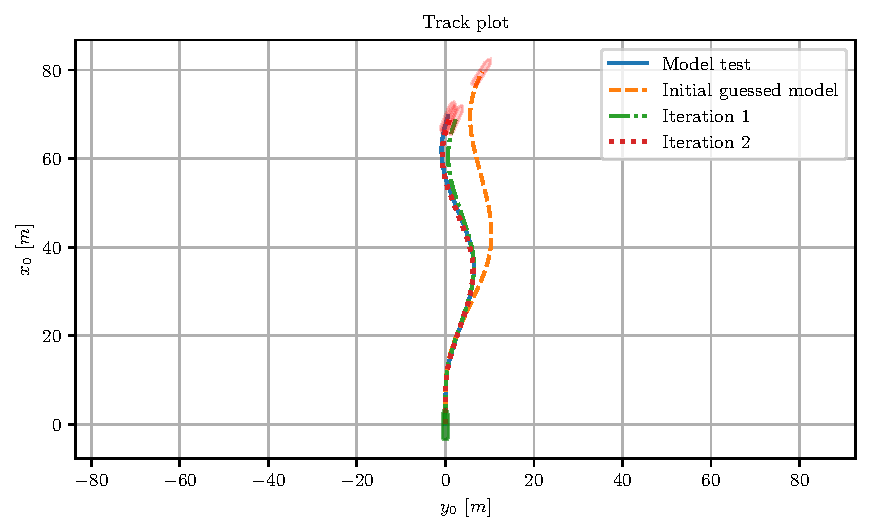
\includegraphics[width=\textwidth]{kappa/images/0.pdf}
    \caption{Simulation with: initial model, first and second iteration of the PIT}
    \label{\detokenize{01.01_method:iterations}}
\end{figure}

\subsection{Inverse dynamics and regression}
\label{\detokenize{03.01_inverse_dynamics:inverse-dynamics-and-regression}}\label{\detokenize{03.01_inverse_dynamics::doc}}
\sphinxAtStartPar
Each manoeuvring model has some hydrodynamic functions \(X_D(u,v,r,\delta,thrust)\), \(Y_D(u,v,r,\delta,thrust)\), \(N_D(u,v,r,\delta,thrust)\) that are defined as polynomials. The hydrodynamic derivatives in these polynomials can be identified with force regression of measured forces and moments. The measured forces and moments are usually taken from Captive Model Tests (CMT), Planar Motion Mechanism (PMM) tests or Virtual Captive Tests (VCT). When the ship is free in all degrees of freedom, as in the present model tests, only
motions are recorded however. Hence, forces and moments causing ship motions need to be estimated by
solving the inverse dynamics problem.
The inverse dynamics is solved by restructuring the system equation (\autoref{equation:02.01_VMMs:eqqsystem}) to get the hydrodynamics functions on the left-hand side. If the mass and inertia of the ship including added masses: \(X_{\dot{u}}\), \(Y_{\dot{v}}\), \(Y_{\dot{r}}\), \(N_{\dot{v}}\) and \(N_{\dot{r}}\), are known, the forces in Prime system can be calculated using \autoref{equation:03.01_inverse_dynamics:eqxd}, \autoref{equation:03.01_inverse_dynamics:eqyd} and \autoref{equation:03.01_inverse_dynamics:eqnd}.
These forces can be used to regress the hydrodynamic derivatives using the Ordinary Least Square (OLS) method. 
\begin{equation}\label{equation:03.01_inverse_dynamics:eqxd}
\begin{split}\displaystyle \operatorname{X_{D}'}{\left(u',v',r',\delta,thrust' \right)} = - X_{\dot{u}}' \dot{u}' + \dot{u}' m' - m' r'^{2} x_{G}' - m' r' v'\end{split}
\end{equation}\begin{equation}\label{equation:03.01_inverse_dynamics:eqyd}
\begin{split}\displaystyle \operatorname{Y_{D}'}{\left(u',v',r',\delta,thrust' \right)} = - Y_{\dot{r}}' \dot{r}' - Y_{\dot{v}}' \dot{v}' + \dot{r}' m' x_{G}' + \dot{v}' m' + m' r' u'\end{split}
\end{equation}\begin{equation}\label{equation:03.01_inverse_dynamics:eqnd}
\begin{split}\displaystyle \operatorname{N_{D}'}{\left(u',v',r',\delta,thrust' \right)} = I_{z}' \dot{r}' - N_{\dot{r}}' \dot{r}' - N_{\dot{v}}' \dot{v}' + \dot{v}' m' x_{G}' + m' r' u' x_{G}'\end{split}
\end{equation}
\sphinxAtStartPar
An example of forces calculated with inverse dynamics from motions in a turning circle test can be seen in \hyperref[\detokenize{03.01_inverse_dynamics:fig-inverse}]{Fig.\@ \ref{\detokenize{03.01_inverse_dynamics:fig-inverse}}}. The forces have been converted to SI units.

\begin{figure}[H]
    \centering
    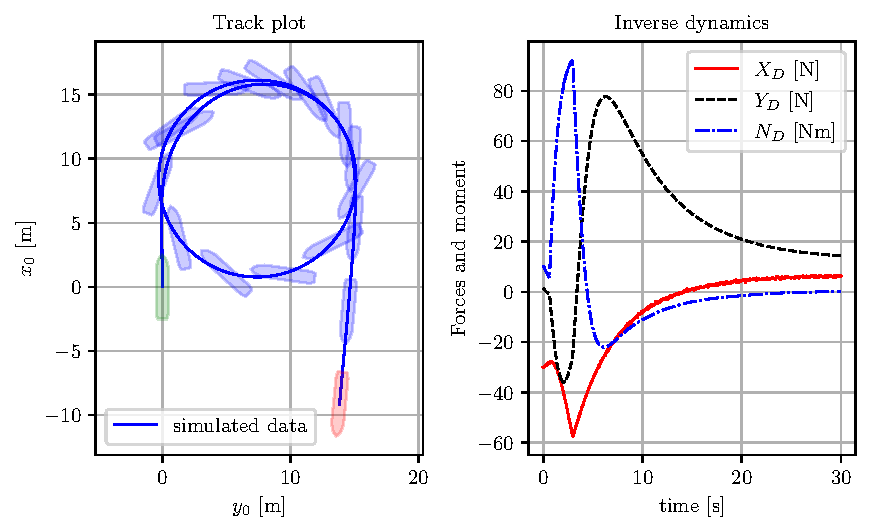
\includegraphics[width=\textwidth]{kappa/images/1.pdf}
    \caption{Example of forces and moments calculated with inverse dynamics on data from a turning circle test.}
    \label{\detokenize{03.01_inverse_dynamics:fig-inverse}}
\end{figure}

\subsection{Data cleaning}
\label{sec:datacleaning}
It is possible to do an exact parameter identification on perfect (simulated) data with no noise (see Paper \ref{pap:daiyong} and \ref{pap:pit}). However, such data from physical experiments does not exist in reality. The measured data will always contain process noise and measurement noise. In order to mitigate this, the data is preprocessed using the EKF and RTS smoother which are both presented below.

EKF is an extension of the Kalman Filter (KF) to work on nonlinear systems such as the VMMs. The basic idea is that noise can be disregarded if it does not make sense from a physical point of view. If noisy measurement data were perfectly correct, this would mean that the ship has many vibrations that must have originated from tremendous forces, considering the large mass of the ship. The prior understanding of the dynamics suggests that these forces are not present. Therefore, the noise should be considered as measurement noise and should be removed. Low-pass filtering is a common way to remove noise, where motions above some cut-off frequencies are regarded as unphysical measurement noise. The problem with low-pass filter is that it is hard to know what cut-off frequency to choose, either too low: removing part of the signal, or too high: keeping some unfiltered measurement noise in the data. The Kalman filter has a system model that continuously estimates the system’s state that runs in parallel with the measurement data. The filter estimates the current state as a combination of the measurement data and the system model estimate based on belief in the data and the model. If the data has low noise, the estimate turns toward that data. Conversely, if the model gives very good predictions, then that estimate turns towards the model.
The system’s inverse dynamics require the entire states, including positions, velocities, and accelerations, to be known. Only positions are known from the measurements, which means that velocities and accelerations are hidden states that the EKF should estimate.

The EKF is recursive and can be run online, continuously making new estimates as new measurements arrive. The EKF uses passed measurements to estimate states in the near future. This property is helpful for online applications such as  autopilots or autonomous ships. This restriction is  unnecessary for the PIT on already existing data where a whole time series of existing measurements is available. The fact that both past and future data are known can be used to improve the filter. An EKF filter can include future time steps by adding a smoother after the filter. The PIT uses a Rauch Tung Striebel (RTS) smoother \cite{rauch_maximum_1965}, which is an algorithm that runs the EKF backward to also account for future time steps.



%%%%%%%%%%%%%%%%%%%%%%%%%%%%%%%
%%%%%%%%%%%%%%%%%%%%%%%%%%%%%%%
\chapter{Results\label{ch:results}}
%%%%%%%%%%%%%%%%%%%%%%%%%%%%%%%
This chapter presents a summary of the appended papers, including research activities
and a selection of the important results, and highlights the main achievements.

\section{Summary Paper \ref{pap:rolldamping}}
\subsection*{"\nameref{pap:rolldamping}"}
In Paper \ref{pap:rolldamping}, time series data from 250 roll decay tests (see Fig. \ref{fig:ship_types}) assembled from the Maritime Dynamics Laboratory at SSPA Sweden AB (\href{www.sspa.se}{www.sspa.se}) are used to investigate the roll motion model. 

\begin{figure}[H]
    \centering
    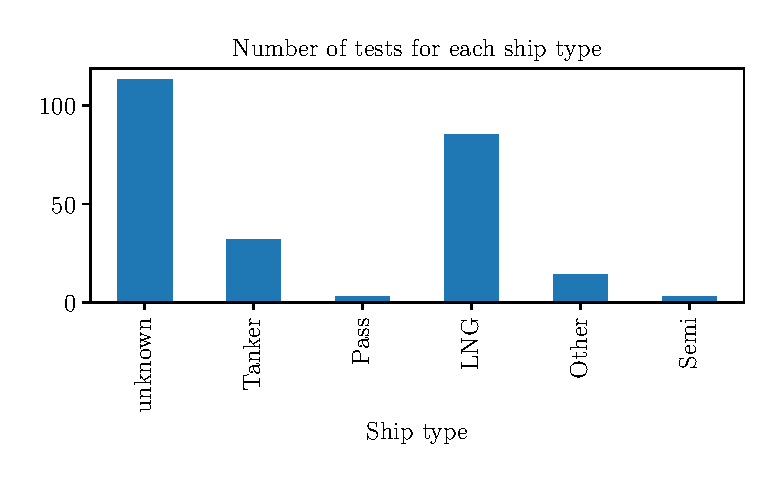
\includegraphics[width=0.5\columnwidth]{kappa/images/ship_types.eps}
    \caption{Number of tests per ship type}
    \label{fig:ship_types}
\end{figure}

\noindent Parameters in the linear (Eq.\ref{eq:roll_decay_equation_himeno_linear}), quadratic (Eq.\ref{eq:roll_decay_equation_himeno_quadratic_b}) and cubic (Eq.\ref{eq:roll_decay_equation_cubic}) roll motion model are identified using the roll motion PIT (see section \ref{sec:PIT_roll}). The investigation shows that the quadratic damping model has almost the same accuracy as the cubic model. The ''integration approach'' (see section \ref{sec:integration_approach}) to PIT roll motion, produces the most accurate models compared to the ''derivation approach'' (see section \ref{sec:derivation_approach}).

\subsection{Generic roll damping model}
\label{sec:genericrolldampingmodel}
A serial grey-box model for ship roll damping (see Fig.\ref{fig:greyrolldamping}) is also developed in Paper \ref{pap:rolldamping}. 
This is expanding the system identification, not only focusing on one ship, but rather all modern ships, by a prediction model of the damping coefficients from the PIT applied on a whole database of roll decay tests. 
Simplified Ikeda's (SI) method \cite{kawahara_simple_2011} is used as the white box model, which is combined with a following black-box correction model.

\begin{figure}[H]
    
    \centering
    \begin{tikzpicture}[node distance=2cm]
    \node (white-box) [white-box] {Simplified Ikeda};
    \node (B_BK) [io, right of=white-box, xshift=0.90cm, yshift=1.5cm] {$\hat{B_{BK}}$};
    \node (B_E) [io, right of=white-box, xshift=0.75cm, yshift=0.75cm] {$\hat{B_{E}}$};
    \node (B_F) [io, right of=white-box, xshift=0.75cm, yshift=0cm] {$\hat{B_{F}}$};
    \node (B_L) [io, right of=white-box, xshift=0.75cm, yshift=-0.75cm] {$\hat{B_{L}}$};
    \node (B_W) [io, right of=white-box, xshift=0.75cm, yshift=-1.5cm] {$\hat{B_{W}}$};
    
    
    \node (black-box) [black-box, right of=B_F, xshift=0.75cm] {Black-box};
    \draw [arrow] (white-box) -- (B_BK);
    \draw [arrow] (white-box) -- (B_E);
    \draw [arrow] (white-box) -- (B_F);
    \draw [arrow] (white-box) -- (B_L);
    \draw [arrow] (white-box) -- (B_W);
    
    \draw [arrow] (B_BK) -- (black-box);
    \draw [arrow] (B_E)  -- (black-box);
    \draw [arrow] (B_F)  -- (black-box);
    \draw [arrow] (B_L)  -- (black-box);
    \draw [arrow] (B_W)  -- (black-box);
    
    
    \node (B) [io, right of=black-box, xshift=0.75cm, yshift=0cm] {$B$};
    \draw [arrow] (black-box)  -- (B);
    
    \end{tikzpicture}
    \caption{Grey-box model to predict roll damping}
    \label{fig:greyrolldamping}
\end{figure}

\noindent The roll damping data set, obtained from the roll motion investigation, is used to train the black-box part of the grey-box model. The black-box correction model of the output components from the SI method are shown in (Eq.\ref{eq:polynom_correction}),
\begin{equation} \label{eq:polynom_correction}
\hat{B_{e}} = 1.106 \hat{B_{BK}} - 0.9124 \hat{B_{E}} + 4.282 \hat{B_{F}} + 0.7457 \hat{B_{L}} + 0.1844 \hat{B_{W}} + 0.004999 \phi_{a} - 0.0005097
\end{equation}


\noindent Large corrections of the skin friction damping $\hat{B_F}$ and wave damping $\hat{B_W}$ are suggested by this expression. This is because the SI method is not very accurate for this dataset, where most of the ships in the dataset exceed the limits of the method. A pure black-box model is also devloped in Paper \ref{pap:rolldamping} (see Eq.\ref{eq:polynom_complex}),
\begin{equation} \label{eq:polynom_complex}
\begin{aligned} 
 \hat{B_{e}} = - 0.02578 A_{0} V - 0.02705 BK_{B} V + \\ 
 0.008993 BK_{L} V - 0.03191 C_{b} V - 0.2028 OG V + \\ 
 0.003472 V^{2} + \\ 
 0.004234 V \hat{\omega_{0}} - 0.002591 V \phi_{a} - 0.008384 V beam + \\ 
 0.05048 V + \\ 
 0.007814 \hat{\omega_{0}}^{2} + \\ 
 0.03882 \hat{\omega_{0}} \phi_{a} - 0.001069 \\ 
 \end{aligned}
\end{equation}


\noindent The grey-box model and the black-box model above, have about the same accuracy when performing cross-validation on the roll damping dataset.

\section{Summary Paper \ref{pap:daiyong}}
\subsection*{"\nameref{pap:daiyong}"}
Least Square Support Vector Regression (LS-SVR) \cite{brereton_support_2010} is used in Paper \ref{pap:daiyong} to identify the parameters in the AVMM.  
The data is taken from experimental tests on a lake using a ship model with a scale of 50:1. The configuration of sensors and equipment for the experiment is shown in Fig.\ref{fig:cthmodel}.  
\begin{figure}[H]
    \centering
    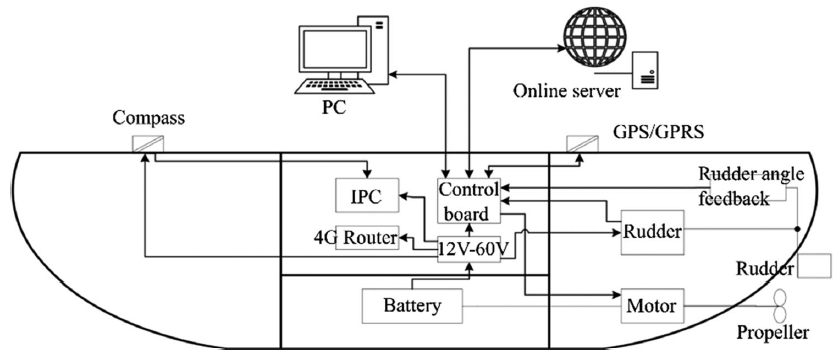
\includegraphics[width=\textwidth]{kappa/images/cth_model.png}
    \caption{Configuration of sensors and equipment for the experimental tests.}
    \label{fig:cthmodel}
\end{figure}
\noindent The hydrodynamic derivatives of the AVMM are identified almost perfectly when applied on data from simulations with MSS toolbox Mariner \cite{tristan_matlab_2009}. The PIT does however not work at all when applied on the data obtained from the lake experiments as seen in Fig.\ref{fig:daiyong_extrapolation}. 

\begin{figure}[H]
    \centering
    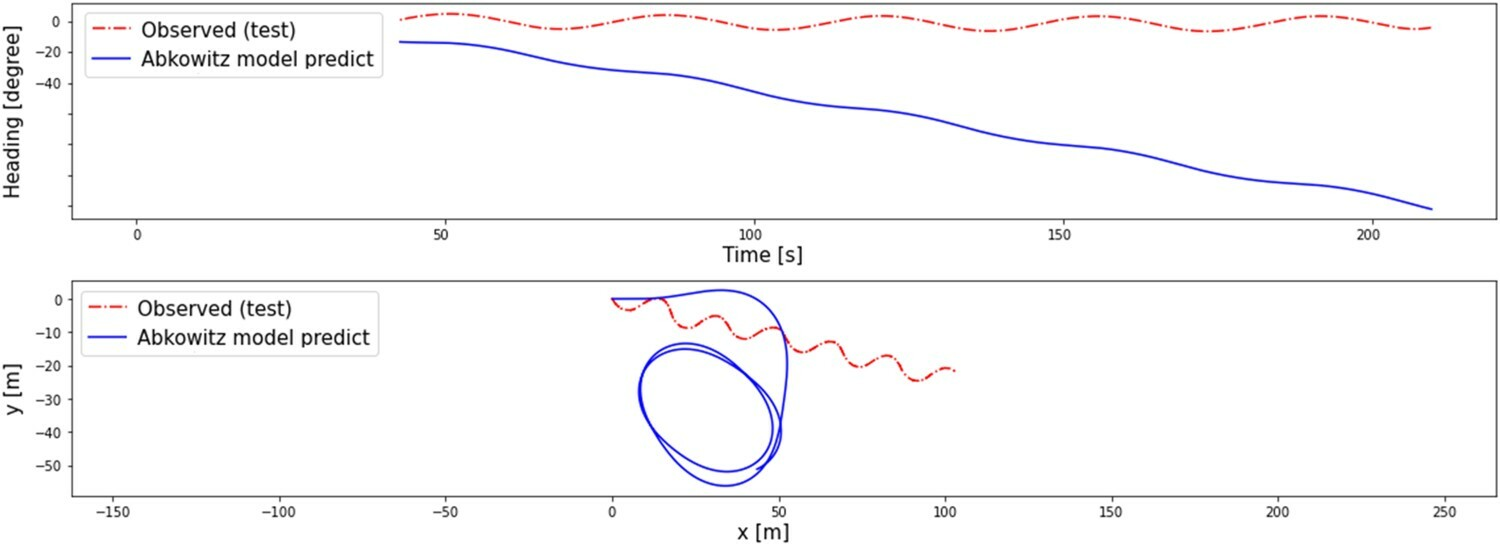
\includegraphics[width=\linewidth]{kappa/images/daiyong_extrapolation.jpeg}
    \caption{Prediction with AVMM of zigzag lake experiments.}
    \label{fig:daiyong_extrapolation}
\end{figure}

\noindent The PIT is very sensitive to noise due to the differentiation that needs to be conducted to calculate velocities and yaw rate from the measured position and heading. The PIT works better if the data is first cleaned using a proposed preprocessing algorithm together with a Kalman Filter (KF). The simulations with the identified model and the experiments are however still not in very good agreement.     

\section{Summary Paper \ref{pap:pit}}
\subsection*{"\nameref{pap:pit}"}
A new method for System Identification of ship manoeuvring dynamics is developed in Paper \ref{pap:pit}. The system model for the ship manoeuvring is assumed to be represented by a VMM (see Section \ref{sec:VMM}). The appropriate VMM for the specific ship and data is selected from a set of candidate VMMs, with varying complexity as a function of its number of hydrodynamic derivatives. The appropriate VMM is selected to give a robust model that can make predictions outside the domain covered by the available training data. A cross validation scheme is proposed to be used in the selection. In this scheme, the validation set has larger drift angles, yaw rates and rudder angles compared to the training set as seen in the example in Fig.\ref{fig:cross_validation}.
\begin{figure}[H]
    \centering
    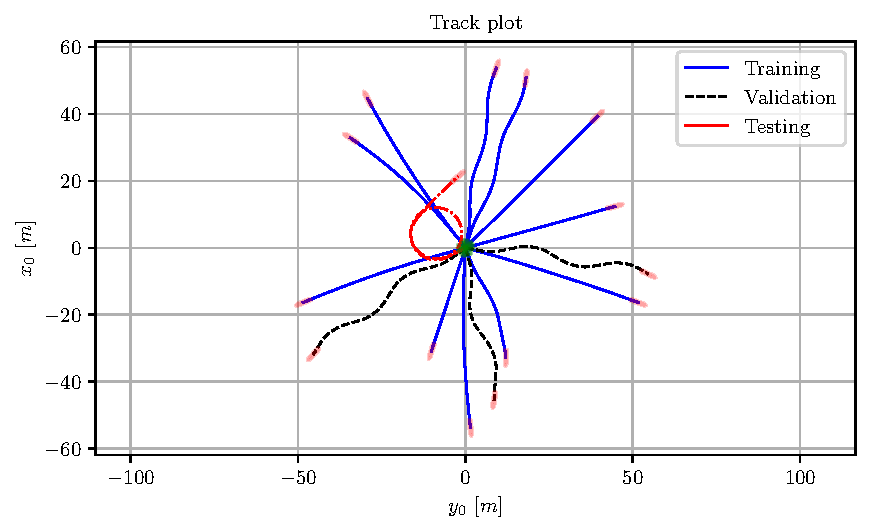
\includegraphics[width=\linewidth]{kappa/images/3.pdf}
    \caption{wPCC training, validation and testing datasets.}
    \label{fig:cross_validation}
\end{figure}
\noindent A new PIT for VMMs (see Section \ref{sec:PIT_VMM}), with large focus on the data cleaning, is also proposed in Paper \ref{pap:pit}. This PIT is investigated together with the method to select a appropriate and robust VMM for two very different cases. The wPCC test case which is a twin screw Pure Car Truck Carrier and the KVLCC2 being a single screw Very Large Crude Carrier.    
\begin{itemize}
    \item The new method can predict turning circle manoeuvres with less than 5 \% error in advance and tactical diameter for the wPCC and KVLCC2 test cases. Track plot of the wPCC result is shown in Fig.\ref{fig:turning_circle_wpcc}.
    
    \item It is shown that the hydrodynamic derivatives within a VMM can be identified exactly at ideal conditions with no measurement noise and a perfect estimator.
    
    \item It is shown that the proposed prepossessing of measurement data with EKF + RTS run in iteration with initial guess from semi-empirical formulas, is better than using low-pass filters for cleaning.
    
\end{itemize}

\begin{figure}[H]
    \centering
    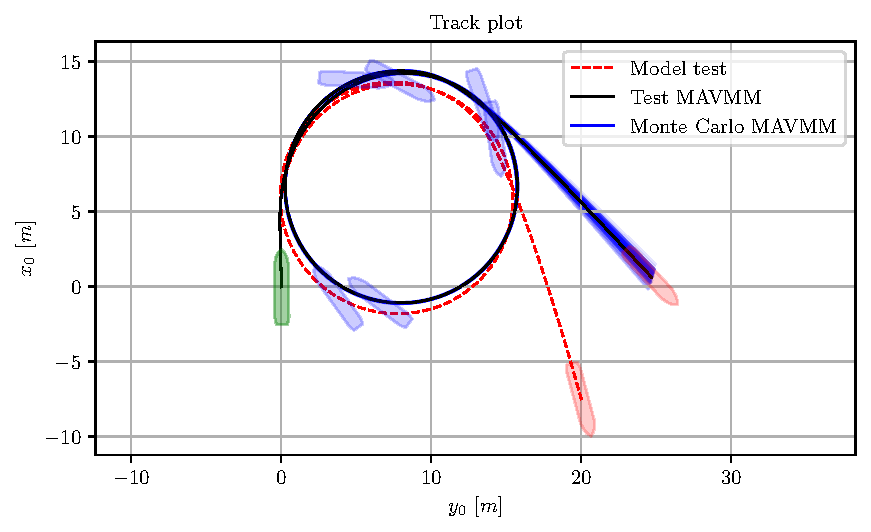
\includegraphics{kappa/images/10.pdf}
    \caption{Track plots of the turning circle test case for wPCC from Model test and simulation (Test). Also simulations with alternative realizations of the regression (Monte Carlo) are shown in this figure.}
    \label{fig:turning_circle_wpcc}
\end{figure}





%%%%%%%%%%%%%%%%%%%%%%%%%%%%%%%
%%%%%%%%%%%%%%%%%%%%%%%%%%%%%%%
\chapter{Conclusions\label{ch:conclusions}}
%%%%%%%%%%%%%%%%%%%%%%%%%%%%%%%
The PIT ''integration approach'' produced better models than the ''derivation approach'' for the roll motion models in Paper \ref{pap:rolldamping}. The ''integration approach'' is very slow and relies on optimization that may or may not converge.
The numerical differentiation that was used in Paper \ref{pap:rolldamping} to estimate the velocities and accelerations, is believed to be the main cause of the poor performance of the much faster and more reliable ''derivation approach''. The introduction of EKF + RTS smoother in the PIT presented in Paper \ref{pap:pit}, solves this issue, with good results for the ''derivation approach''.

The SI method, being the white-box physical model in the grey-box model in Paper \ref{pap:rolldamping} has about the same accuracy as the corresponding black-box model, which means that the white-box model is adding very little value, due to poor performance of SI method outside its limits.

 

   
%%%%%%%%%%%%%%%%%%%%%%%%%%%%%%%
%%%%%%%%%%%%%%%%%%%%%%%%%%%%%%%
\chapter{Future work\label{ch:future_work}}
%%%%%%%%%%%%%%%%%%%%%%%%%%%%%%%

\subsubsection*{New generic roll damping model}
The PIT of the roll motion models applied on 250 roll-decay tests that was investigated in Paper \ref{pap:rolldamping} produced a roll damping database for modern ship types. A grey-box model and a black-box model as described in Section \ref{sec:genericrolldampingmodel} was developed from this database. The prediction accuracy of these models were not very good and should be improved. This is important, especially since the SI method, being the state of art white-box physical model for roll damping, was found to be outside its limits for the ships in the database. This implies that there is a need for a new roll damping prediction method for modern ships.  

\renewcommand\bibname{References}
\printbibliography[heading=bibintoc]

%  \end{refsection}

\cleardoublepage

%\printbibliography[heading=subbibintoc] % biblatex bibliography


% % % Preparations before Part II. In this part one chapter = one paper

\renewcommand{\chaptername}{Paper}
                              % write 'Paper' instead of 'Chapter' in the title

\setcounter{chapter}{0}       % reset chapter numbers after Part I


% Fix hyperlinks to chapters/papers after chapter counter reset, see
% http://tex.stackexchange.com/a/6099
\renewcommand\theHchapter{appendedPaper.\arabic{chapter}}

\renewcommand{\thesection}{\arabic{section}}
                              % exclude chapter number from section number
                              % Figures, Tables, etc are still prefixed by chapter number.
                              % For algorithms numbering see definition of
                              % \newfloat{algorithm} above.

\newcommand{\paper}[7]
% #1 Paper Title
% #2 Short Title for page headers (ToC has the full title)
% #3 Label for later (or earlier) \ref:s
% #4 Authors
% #5 Where published
% #6 Comment (like "reprinted with a kind permission" and "reformatted for uniformity")
% #7 File to input
{
  \chapter{#1\label{#3}}      % Title as Chapter
  \chaptermark{#2}            % Short title for the page header
  \thispagestyle{empty}       % no page numbers
  {\Large #4}\par             % authors
  \vspace{1cm}
  \noindent\emph{\Large #5}\par % where published
  \vspace{3cm}
  \noindent\emph{\Large #6}   % Comment
%  \cleardoublepage            % skip back side of the page
%  \thispagestyle{plain}       % no header above paper title
%  \begin{center}
%    {\Large \bfseries Paper~\thechapter. #1}\par % title again
%    \vspace{1pc}
%    #4 \par                   % authors again
%    \vspace{3pc}
%  \end{center}
%  \begin{refsection}          % start of biblatex's refsection for sub-bibliography
%  \input{#7}                  % paper itself, starting from abstract (no title)
%  \printbibliography[heading=subbibintoc] % biblatex bibliography
%  \end{refsection}            % end of biblatex refsection
}

\newcommand{\reformatted}{The paper was reformatted for uniformity, but otherwise is unchanged.}

\addtocontents{toc}{\cftpagenumbersoff{chapter}}

\setcounter{part}{1}
\part{Appended papers}        % in this part one chapter = one paper

% Example of using the command \paper defined above: 
\paper{Analysis of roll damping model scale data}
      {~}
      {pap:rolldamping}
      {\fullcite{alexandersson_analysis_2021}}
      {~}
      {~}

\paper{System identification of {vessel} {manoeuvring} {models}}
      {~}
      {pap:pit}
      {\fullcite{alexandersson_system_2022}}
      {Accepted for publication in Ocean Engineering.}
      {~}

\end{document}
